%----------------------------------------------------------------------------------------
%    PACKAGES AND DOCUMENT CONFIGURATION
%----------------------------------------------------------------------------------------

\documentclass[11pt]{article}

% MARGINS, GEOMETRY, FONTS
\usepackage[a4paper,margin=0.7in]{geometry}  % Adjust page size and margins
\usepackage{lmodern}                       % Latin Modern font (less pixelation in PDF)
\usepackage[T1]{fontenc}                   % Better character encoding
\usepackage[utf8]{inputenc}                % UTF-8 encoding
\usepackage{amsmath,amsthm,amssymb}        % AMS math packages
%\usepackage{mathrsfs}                      % Nice script fonts
\usepackage{mathtools}                     % Extra math goodies
\usepackage{microtype}                     % Better spacing, text aesthetics
\usepackage{tikz}
\usepackage{pgfplots}
\usepackage{placeins}


\pgfplotsset{compat=1.18}
\usepgfplotslibrary{patchplots}
\usetikzlibrary{3d}

\usepackage{mathspec}
\defaultfontfeatures{Mapping=tex-text}
\usepackage{fontspec}
\setmainfont{IBM Plex Serif}

%%% PYTHON CHUNKS
\usepackage{listings}
\usepackage{xcolor}

\definecolor{codegray}{rgb}{0.5,0.5,0.5}
\definecolor{codepurple}{rgb}{0.58,0,0.82}
\definecolor{backcolour}{rgb}{0.95,0.95,0.92}

\lstdefinestyle{pythonstyle}{
    backgroundcolor=\color{backcolour},   
    commentstyle=\color{codegray},
    keywordstyle=\color{blue}\bfseries,
    numberstyle=\tiny\color{gray},
    stringstyle=\color{codepurple},
    basicstyle=\ttfamily\footnotesize,
    breaklines=true,
    captionpos=b,
    keepspaces=true,
    numbers=left,
    numbersep=5pt,
    showspaces=false,
    showstringspaces=false,
    showtabs=false,
    language=Python
}

\lstset{style=pythonstyle}


% CUSTOM HEADER AND FOOTER
\usepackage{fancyhdr}
\pagestyle{fancy}
\fancyhf{}
\lhead{\footnotesize \textsc{Fast-Sweeping \& Path Planning , Hugo Belzil}}
\rhead{\footnotesize \textsc{\thepage}}
\cfoot{\footnotesize \textit{}}
\renewcommand{\headrulewidth}{0.4pt}
\renewcommand{\footrulewidth}{0pt}

% OTHER USEFUL PACKAGES
\usepackage{graphicx}       % For including images
\usepackage{booktabs}       % Nicer horizontal rules in tables
\usepackage{enumerate}      % For customizable lists
\usepackage{xcolor}         % For color in text/equations
\usepackage{hyperref}       % Hyperlinks in the PDF
\hypersetup{
    colorlinks = true,
    linkcolor  = blue,
    citecolor  = magenta,
    urlcolor   = teal
}

% ENVIRONMENTS (THEOREM, DEFINITION, EXAMPLE, ETC.)
\newtheorem{theorem}{Theorem}[section]
\newtheorem{lemma}[theorem]{Lemma}
\newtheorem{prop}[theorem]{Proposition}
\newtheorem{cor}[theorem]{Corollary}

\theoremstyle{definition}
\newtheorem{definition}[theorem]{Definition}
\newtheorem{example}[theorem]{Example}

\theoremstyle{remark}
\newtheorem{remark}[theorem]{Remark}

% CUSTOM COMMANDS
\newcommand{\R}{\mathbb{R}}
\newcommand{\N}{\mathbb{N}}
\newcommand{\Z}{\mathbb{Z}}
\newcommand{\Q}{\mathbb{Q}}

%----------------------------------------------------------------------------------------
%    TITLE PAGE
%----------------------------------------------------------------------------------------

\begin{document}

\begin{titlepage}
    \centering
    \vspace*{2cm}
    {\huge \bfseries THE FAST-SWEEPING METHOD FOR EIKONAL EQUATIONS \& AN APPLICATION
    TO OPTIMAL CONTROL \par}
    \vspace{1.5cm}
    {\Large \textsc{Hugo Belzil} \par}
    \vspace{0.4cm}
    \textit{MATH 478 - Computational Methods for Applied Mathematics} \\
    \textit{Instructor: Dr.~J.C. Nave} \\
    \textit{Semester: Winter 2025} \\
    \textit{McGill University}
    \vfill
    \vspace{0.8cm}
    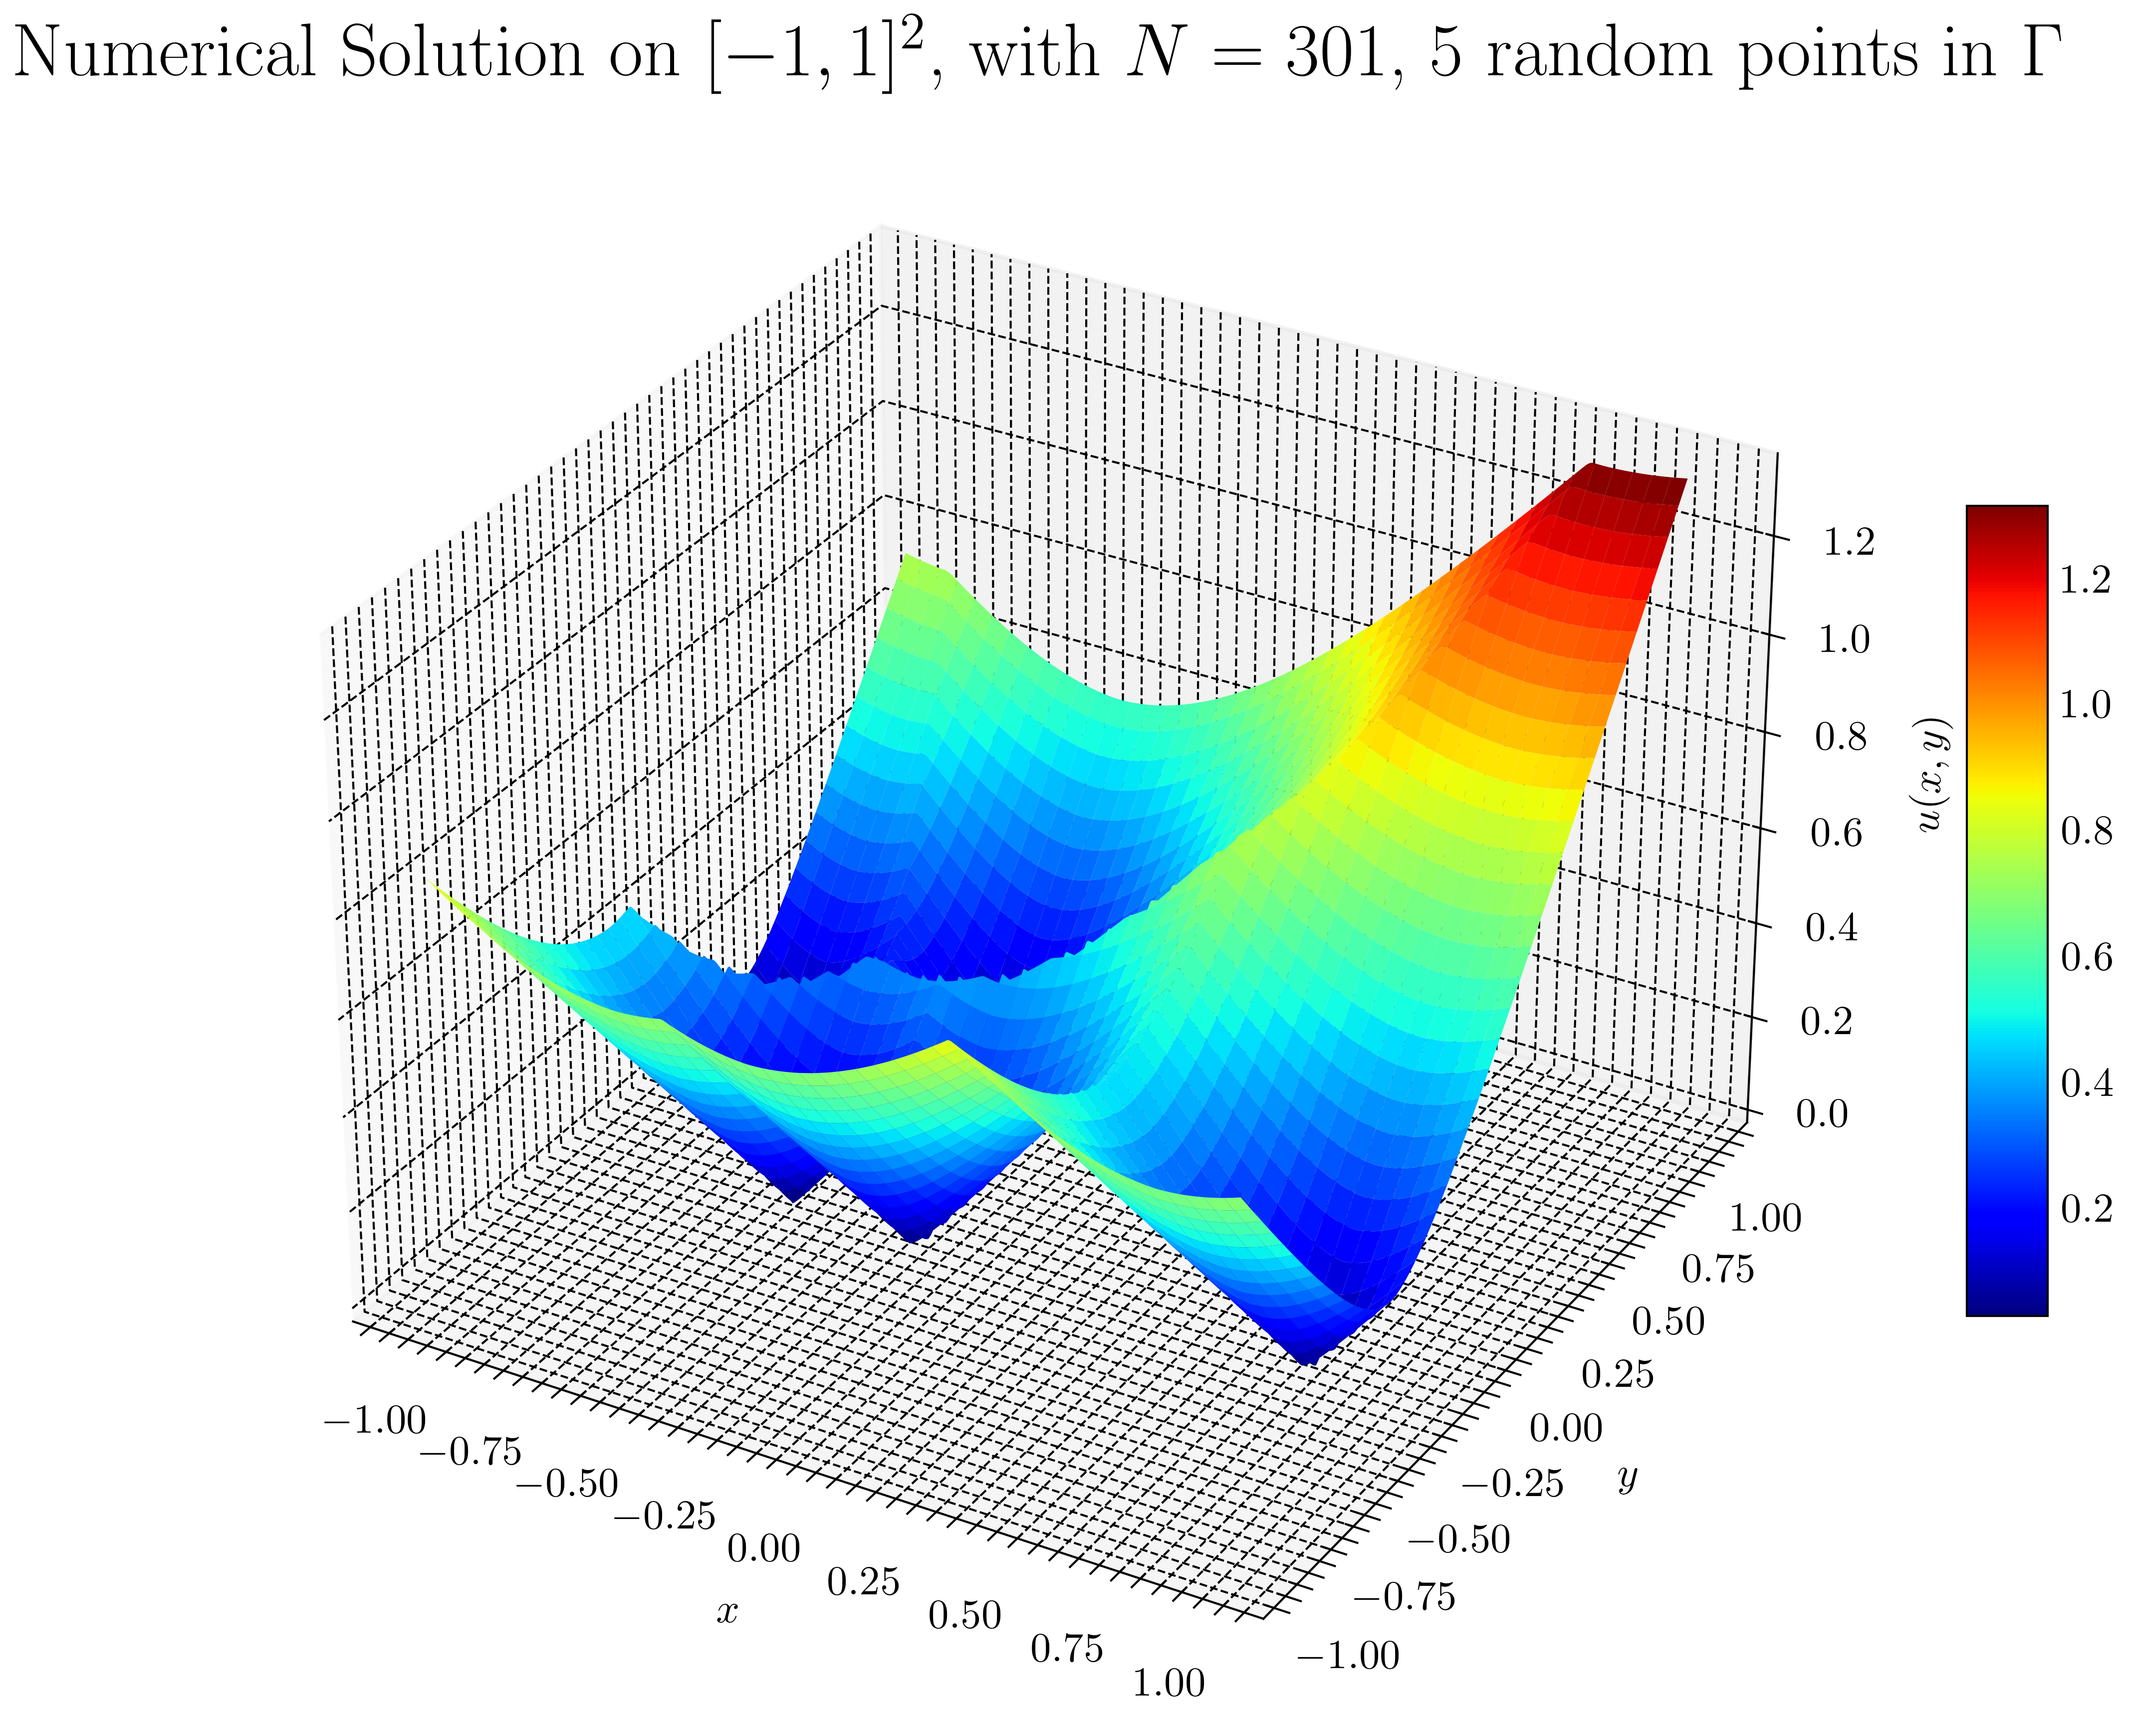
\includegraphics[width=0.7\textwidth]{plots/solution_3d_surface_random5.png} % Replace with your own logo or image
    \vfill
    \vspace{0.8cm}
    {\large \today\par}
\end{titlepage}

%----------------------------------------------------------------------------------------
%    TABLE OF CONTENTS (OPTIONAL)
%----------------------------------------------------------------------------------------

\tableofcontents
\thispagestyle{empty}

\clearpage

\section{Introduction}
%this is where you will describe the problem (e.g. previous work, related work,...) you are solving and the objectives
\label{sec:intro}
The Eikonal equations have several applications across many fields of mathematics, engineering, and others. They are particularly used for solving optimization problems, as we will see in this project. These equations associated to some side-condition, are of the form \\
\begin{equation}
\label{original-eikonal}
    \begin{cases}
        |\nabla u(\vec{x})|=f(\vec{x}) , \quad\vec{x} \in\Omega\\
        u(\vec{x})=\phi(\vec{x}),\quad \vec{x} \in \Gamma \subset \Omega
    \end{cases}
\end{equation}
where $|\cdot|$ denotes the Euclidean norm in $\R^n$, and $u,f,\phi:\R^n\xrightarrow{}\R$. \\

\noindent In this report, we will focus on solving Eikonal equations in 2 space dimensions. We will introduce the discretization and fast-sweeping method proposed by H.Zhao in 2008 \cite{zhao2005}, considering several scenarios for $f(x,y)$ and $\Gamma$, and observing some numerical results. Finally, we will use these results and apply them to an optimal control problem : path planning. The Python implementation of the Fast-Sweeping method and all scripts used in this report are available on GitHub at: 
\href{https://github.com/hugobelzil/eikonal_project}{github.com/hugobelzil/eikonal\_project}.


\section{Theory}
%Introduce the equation and give some details
\subsection{Origins and derivation}
Eikonal equations are common equations, encountered in several fields of the sciences. They first arose in geometric optics problems on the propagation of light waves, the term \textit{eikonal} being a germanization of the greek word \textit{eikon}, meaning "image" or "icon"\cite{wiki-eikonal}. We will see in section (\ref{section_snells_law}) an example where it applies to the refraction of light in changing media. \\

\noindent These equations however arise in several other fields, including optimal control theory and robotics. The solutions of eikonal equations can also be used to compute optimal paths in time, as we will see in section (\ref{path_planning}). \\

\noindent In particular, the differential equation (\ref{original-eikonal}) can be derived from level-set equations, for the propagation of a front for example. If we let the 0-level set of a function $\phi(\vec{x},t)$ represent a curve or a surface moving in space (being a front), we need the function $\phi$ to satisfy the advection equation: \\
\begin{equation}
\label{level_set_equation}
    \phi_t+F(\vec{x})|\nabla \phi| =0
\end{equation} \\
where $F:\vec{x}\rightarrow\R$ represents the velocity at which the point $\vec{x}$ on the curve (or surface) moves. If we restrict $F$ to be strictly positive, we force the curve to move "outward" and extend in space. This assumption allows us the make the ansatz that $\phi$ can be expressed as : $\phi(\vec{x},t)=\psi(\vec{x})-t$. The reason for this is the following : this form allows us to think of $\psi(\vec{x})$ as the arrival time of the curve (or front) to the point $\vec{x}$ in space. Indeed, recall that the curve is described as the 0-level set of $\phi(\vec{x},t)$. We can now plug-in this ansatz into (\ref{level_set_equation}) and get: \\
\begin{align*}
    & (\psi(\vec{x})-t)_t+F|\nabla(\psi(\vec{x})-t)|=0 \\
    &\implies-1 +F|\nabla\psi| = 0 \\
    &\implies |\nabla\psi|=\frac{1}{F}
\end{align*} \\
\noindent which indeed gives an Eikonal equation. In the front-propagation context, we can hence interpret the solution as the following : the arrival times $\psi$ in space of a front starting at a point $\gamma$ and propagating in a medium with speed $F$ must solve the eikonal equation
\begin{equation*}
    |\nabla\psi(\vec{x})|=\frac{1}{F(\vec{x})}, \quad \psi(\gamma)=0
\end{equation*}
When $F\equiv1$, the front is moving through a uniform media, at the same speed everywhere. Hence, we can view $\psi$ as the distance to $\gamma$ (see section \ref{section_on_distance}). In the analysis above, we let $\gamma$ be a single point in space, but the front could also originate from a curve, or several points in space, as we will see later in this report.

\subsection{Distance function in 2D}
\label{section_on_distance}
An important application of Eikonal functions is the computation of Euclidean distances in $\R^n$. In particular, let us consider the following problem : suppose that we are given a  finite set of points $\Gamma = \{\gamma^{(1)},\dots,\gamma^{(m)}\}$, and for each $\textbf{x}=(x,y)$ in our computational domain, we would like to compute the shortest distance to $\Gamma$. Hence, we would like to have a function $d(x,y)$ such that
\begin{equation}
\label{min-problem}
    d(\textbf{x}) = \min_{\gamma \in \Gamma}\|\textbf{x}-\gamma\|_2
\end{equation}
Consider this problem in $\R^2$, if we let $(x,y)$ such that its closest point in $\Gamma$ is some point $\gamma^{*}=(\gamma_1,\gamma_2)$, which is the unique minimizer of \eqref{min-problem}, then:
\begin{gather*}
    d(x,y) = \sqrt{(x-\gamma_1)^2+(y-\gamma_2)^2} \\[10pt] 
    \implies\frac{\partial d}{\partial x}=\frac{x-\gamma_1}{\sqrt{(x-\gamma_1)^2+(y-\gamma_2)^2}}, \quad 
    \frac{\partial d}{\partial y}=\frac{y-\gamma_2}{\sqrt{(x-\gamma_1)^2+(y-\gamma_2)^2}} \\[10pt] 
    \implies |\nabla d(x,y)| = \sqrt{\Bigg(\frac{\partial d}{\partial x}\Bigg)^2 + \Bigg(\frac{\partial d}{\partial y}\Bigg)^2}=1
\end{gather*}
Indeed, $d(x,y)$ solves the Eikonal equation where $f(x,y) \equiv 1$, and naturally we have $d(x,y)=0$ where $(x,y)\in\Gamma$ (the distance to the boundary is 0 when the point lies on the boundary).

\vspace{5pt}

\noindent Note that we made the important assumption that $\gamma^{*}$ was the only minimizer of (\ref{min-problem}). However, if $\text{card}|\Gamma|\geq2$, then there exist points in $\R^2$ for which (\ref{min-problem}) does not admit a single minimizer, but rather infinitely many. In this case, $d(x,y)$ becomes non-differentiable at these points, which will be discussed in our analysis.
\section{Numerical methods}
\subsection{Discretization and scheme}
%this is where you present your numerical method/scheme. You may additionally put accuracy, stability in here. Also talk about the implementation details here.
H. Zhao proposed the fast-sweeping method in \cite{zhao2005} to solve Eikonal equations numerically. He proposed the following discretization, which uses Gauss-Seidel iterations. In 2 dimensions, given a space step $h$, the scheme is:

\begin{equation*}
    ((u_{i,j}-u_{xmin})^{+})^2+((u_{i,j}-u_{ymin})^{+})^2 = f_{i,j}^{2}h^2
\end{equation*}

\noindent where
\begin{itemize}
    \item $(x)^{+} = \max(x,0)$
    \item $u_{i,j}\approx u(ih,jh)$, $u_{xmin} = \min\{u_{i-1,j},u_{i+1,j}\}$ and $u_{ymin} = \min\{u_{i,j-1},u_{i,j+1}\}$
\end{itemize}

\noindent Figure (\ref{fig:graph_discretization}) shows the dependence of $u_{ij}$ on its neighbouring points during an update. The updates of the points $u_{i,j}$ must be done by "sweeping" the domain in all 4 possible directions (or $2^d$ directions in $\mathbb{R}^d$), after having initialized a grid. Although the order of the sweeps does not matter, the sweeps in 2 dimensions can be done as follows, assuming a square domain:
\begin{itemize}
    \item \textbf{Sweep 1 : } Start from the bottom-left corner of the domain, updating the points from left to right. Hence, the last point updated is the top-right corner one.
    \item \textbf{Sweep 2 : } Start from the bottom-right corner of the domain, updating the points from right to left. This gets us to the last point updated being the top-left corner one.
    \item  \textbf{Sweep 3 : } Start from the top-left corner of the domain, updating from left to right. Similarly, the last point to be updated is the bottom-right corner one.
    \item \textbf{Sweep 4 : } Last possible direction. Start from top-right corner of the domain, updating the points from right to left. The last point to be updated is the bottom left corner.
\end{itemize}

\begin{figure}[h!]
    \centering
    \begin{tikzpicture}
        % Draw the grid points
        \foreach \x in {0,1,2} {
            \foreach \y in {0,1,2} {
                \filldraw (\x,\y) circle (3pt);
            }
        }

        % Highlight the center point (i,j)
        \filldraw[red] (1,1) circle (2pt) node[above right] {$(i,j)$};

        % Draw the stencil neighbors
        \filldraw[blue] (0,1) circle (2pt) node[left] {$(i-1,j)$};
        \filldraw[blue] (2,1) circle (2pt) node[right] {$(i+1,j)$};
        \filldraw[blue] (1,0) circle (2pt) node[below] {$(i,j-1)$};
        \filldraw[blue] (1,2) circle (2pt) node[above] {$(i,j+1)$};

        % Draw lines connecting the stencil points
        \draw[thick] (1,1) -- (0,1);
        \draw[thick] (1,1) -- (2,1);
        \draw[thick] (1,1) -- (1,0);
        \draw[thick] (1,1) -- (1,2);
    \end{tikzpicture}
    \caption{Discretization for the Fast-Sweeping method in 2D}
    \label{fig:graph_discretization}
\end{figure}

\noindent Hence, a full iteration of the scheme can be described as follows:
\begin{itemize}
    \item \textbf{(1)} Initialize the computational domain by setting all points to a large value $M$ (this value should be larger than the largest value of the solution $u$ in the domain).
    \item \textbf{(2)} Place the boundary conditions $\Gamma=\{\gamma_1,\dots,\gamma_m\}$ on the domain. These points are fixed and should never be updated!
    \item \textbf{(3)} Apply a batch of sweeps to the domain, i.e. sweeps 1 to 4. If needed, sweep again the domain until convergence is met. To monitor convergence, compute at the $k$-th sweep $E = \max\limits_{i,j} \left| u_{i,j}^{(k)} - u_{i,j}^{(k-1)} \right|$ where $u_ {i,j}^{(k)}$ denotes the solution on the stencil $(i,j)$ after the $k$-th sweep.
\end{itemize}
\noindent During step (\textbf{3}) in the above, one needs to solve the following equation for every point $u_{i,j}$:
\begin{equation}
\label{system_eq}
    [(u_{i,j}-a)^{+}]^2+[(u_{i,j}-b)^{+}]^2=f_{i,j}^2h^2
\end{equation}
\noindent where $a=\min\{u_{i-1,j},u_{i+1,j}\}$ and $b=\min\{u_{i,j-1},u_{i,j+1}\}$. The solution to (\ref{system_eq}) is given by:
\begin{equation*}
    \bar{u}=\begin{cases}
        \min\{a,b\}+f_{i,j}h & \text {if }|a-b|\geq f_{i,j} \\
        \frac{a+b+\sqrt{2f_{i,j}^2h^2-(a-b)^2}}{2} & \text {if }|a-b|< f_{i,j}
    \end{cases}
\end{equation*} \\
\noindent Finally, $u_{ij}\leftarrow\min\{u_{ij},\bar{u}\}$.


\subsection{Properties of the Fast-Sweeping method}
We report in this section several properties of the fast-sweeping method.
\begin{prop}[\textbf{Monotonicity of the scheme}]
The fast-sweeping scheme in decreasing in the sweeps : $\forall{}\ i,j:u^{(k)}_{ij}-u^{(k-1)}_{ij}\leq0$
\end{prop}
\begin{prop}[\textbf{Number of sweeps and accuracy for distance functions*}]
\label{prop_distance_functions}
    For the distance function in $\R^n$ ($F(x,y)\equiv1$), the fast-sweeping method converges in $2^n$ sweeps. However, this needs to be nuanced and argued differently. \\ \\
    If $|\Gamma|=1$, the scheme converges exactly after $2^n$ sweeps. Hence, in 2 dimensions, a $5^{th}$ sweep will not update the numerical solution $u^h$. In this case, $\|u-u^h\|_{\infty}=\mathcal{O}(|h\log h|)$ \\ \\
    If $|\Gamma|>1$, some points in the computational domain will be at the same distance to at least 2 boundary points in $\Gamma$. This creates an interaction between these boundary points and results in the following. After $2^n$ sweeps, the scheme is still $\mathcal{O}(|h\log h|)$, but further sweeps will still increase the accuracy of the numerical solution (i.e. sweeps still update the numerical solution). In this case, after $2^n+1$ sweeps or more, $\|u-u^h\|_\infty=\mathcal{O}(h)$. \textbf{*REMARK : } this proposition is our understanding from the paper of H. Zhao, but needs to be verified. This will be updated in a future version of this report.
\end{prop}

\begin{prop}[\textbf{*Number of sweeps and accuracy for general equations}]
\label{prop_general_equations}
    In the case where the velocity field $F(x,y)$ is not constant, the number of sweeps needed required to meet convergence depends on the characteristic curves, (and thus, on $F$). \\ \\
    If $|\Gamma|=1$ and $F$ is smooth, this is a special case where we can have an accuracy of order $h\log h$, as for the distance function case above. This is observed non-rigorously later in this report. \\ \\
    If $\Gamma$ and $F$ are such that the solution $u$ develops non-differentiabilities, it appears that the scheme's accuracy becomes of order $\sqrt{h}$. \\
    \textbf{*REMARK : } As for the proposition above, this needs to be verified and will be updated in the future.
\end{prop}

\subsection{Implementation details}
We implement the fast-sweeping method in Python. All scripts are available in the GitHub repository (link the introduction). \\
We replicate domains with the help of a class named \texttt{computational\_domain}
, equipped with the method \texttt{ComputationalDomain(N,a,b,c,d)} which instantiates an object with several attributes, including the attribute \texttt{grid} which is an $N\times N$ Numpy 2D array \cite{numpy}, representing the square $[a,b]\times[c,d]\subset\R^2$. The constructor of the class sets the initial value $M$ mentioned above to 100, but can be chosen by the user.\\
This class is also equipped with the method \texttt{Gamma(coordinates)} which sets the boundary conditions in the domain. \texttt{coordinates} must be a list of 2D coordinates given as a indices, for example \texttt{coordinates = [(0,0), (1,0), (4,4)]}. Note that this method assumes that the coordinates are given in Python indexing. For example, the code below would help create the following domain: \\
\begin{lstlisting}[language=Python, caption=Instance of computational domain, label=lst:fsweep]
from computational_domain import ComputationalDomain
domain = ComputationalDomain(N = 6, a = -1, b = 1, c = -1, d = 1)
domain.Gamma([(0,0), (2,1), (4,3), (1,4)])
print(domain.grid)
\end{lstlisting} \\

$$\[
\begin{bmatrix}
0 & 100 & 100 & 100 & 100 & 100 \\
100 & 100 & 100 & 100 & 0 & 100 \\
100 & 0 & 100 & 100 & 100 & 100 \\
100 & 100 & 100 & 100 & 100 & 100 \\
100 & 100 & 100 & 0 & 100 & 100 \\
100 & 100 & 100 & 100 & 100 & 100
\end{bmatrix}
\]$$ \\


\noindent The code in the repository comes with 2 classes, \texttt{eikonal\_distance\_2D} and \texttt{eikonal\_general\_F}, which help treating distinctly the cases where $F(x,y)\equiv1$ and $F(x,y)\not\equiv1$. Both classes come with a method named \texttt{EikonalSolver()}, both taking as input an object of the class \texttt{computational\_domain} described above. Additionally, the \texttt{EikonalSolver} method from the general function $F$ takes as input the function $F$. An example for both cases is available below. \\

\begin{lstlisting}[language=Python, caption = Instance of an Eikonal Solver for the 2D distance function]
from computational_domain import ComputationalDomain
from solvers.eikonal_distance_2D import EikonalSolver
domain = ComputationalDomain(N = 501, a = -1, b = 1, c = -1, d = 1)
domain.Gamma([(250, 250)])

solver = EikonalSolver(domain = dom)
solver.BatchSweeps(k = 1)
print(solver.grids_after_sweeps[-1])
\end{lstlisting} \\

\noindent In this code above, we solve the Eikonal equation for the distance to the origin over the square $[-1,1]^2$ with $N=501$ grid points. The \texttt{solver} object stores the grid after each sweep, and line 8 allows to access the last grid (after the fourth sweep), which is stored as a Numpy array. The snippet below extends the method to the general function $F$. \\

\begin{lstlisting}[language=Python, caption = Instance of an Eikonal Solver for a general velocity F]
from computational_domain import ComputationalDomain
from solvers.eikonal_general_F_2D import EikonalSolver
domain = ComputationalDomain(N = 501, a = -1, b = 1, c = -1, d = 1)
domain.Gamma([(250, 250)])
eps = 1e-6

def F(x,y):
    return 1 + x**2 + y**2

solver = EikonalSolver(domain = dom, F = F)
solver.SweepUntilConvergence(epsilon = eps, verbose = True)
print(solver.grids_after_sweeps[-1])
\end{lstlisting}

\noindent In this code above, our aim is to solve the Eikonal equation in the same domain, except that $F(x,y)=1+x^2+y^2$. Observe that we now use the method \texttt{SweepUntilConvergence}, which allows us to monitor the convergence after each sweep, and thus avoid unnecessary ones. After each sweep, the method computes the maximum change ($\|\cdot\|_\infty$) between the new grid and the one that had resulted from the previous sweep. If this change is below some threshold \texttt{epsilon}, the method stops. 

\section{Results}
\subsection{Distance functions in 2D}
As argued above in section \ref{section_on_distance}, the Eikonal equation can be used to compute the shortest distance to a boundary $\Gamma \subset \R^n$. Therefore, we test our implementation for the BVP:
\begin{equation}
\label{cone_bvp}
    \begin{cases}
        \|\nabla u(\vec{x})\|_2=1 , \quad\vec{x} \in[-1,1]^2\\
        u(0,0)=0
    \end{cases}
\end{equation}
The solution to this BVP is the 2D cone, given by $u(x,y)=\sqrt{x^2+y^2}$. Therefore, we can easily compare our numerical solution to the analytic one, and study its convergence as well.
For solving numerically (\ref{cone_bvp}), we discretize the square $[-1,1]^2$ uniformly with $N=257 \implies h \approx 0.0078$. The numerical solution converges after exactly 4 sweeps, as outlined by proposition (\ref{prop_distance_functions}). \\

\begin{figure}[h!]
    \centering
    \begin{minipage}{0.48\linewidth}
        \centering
        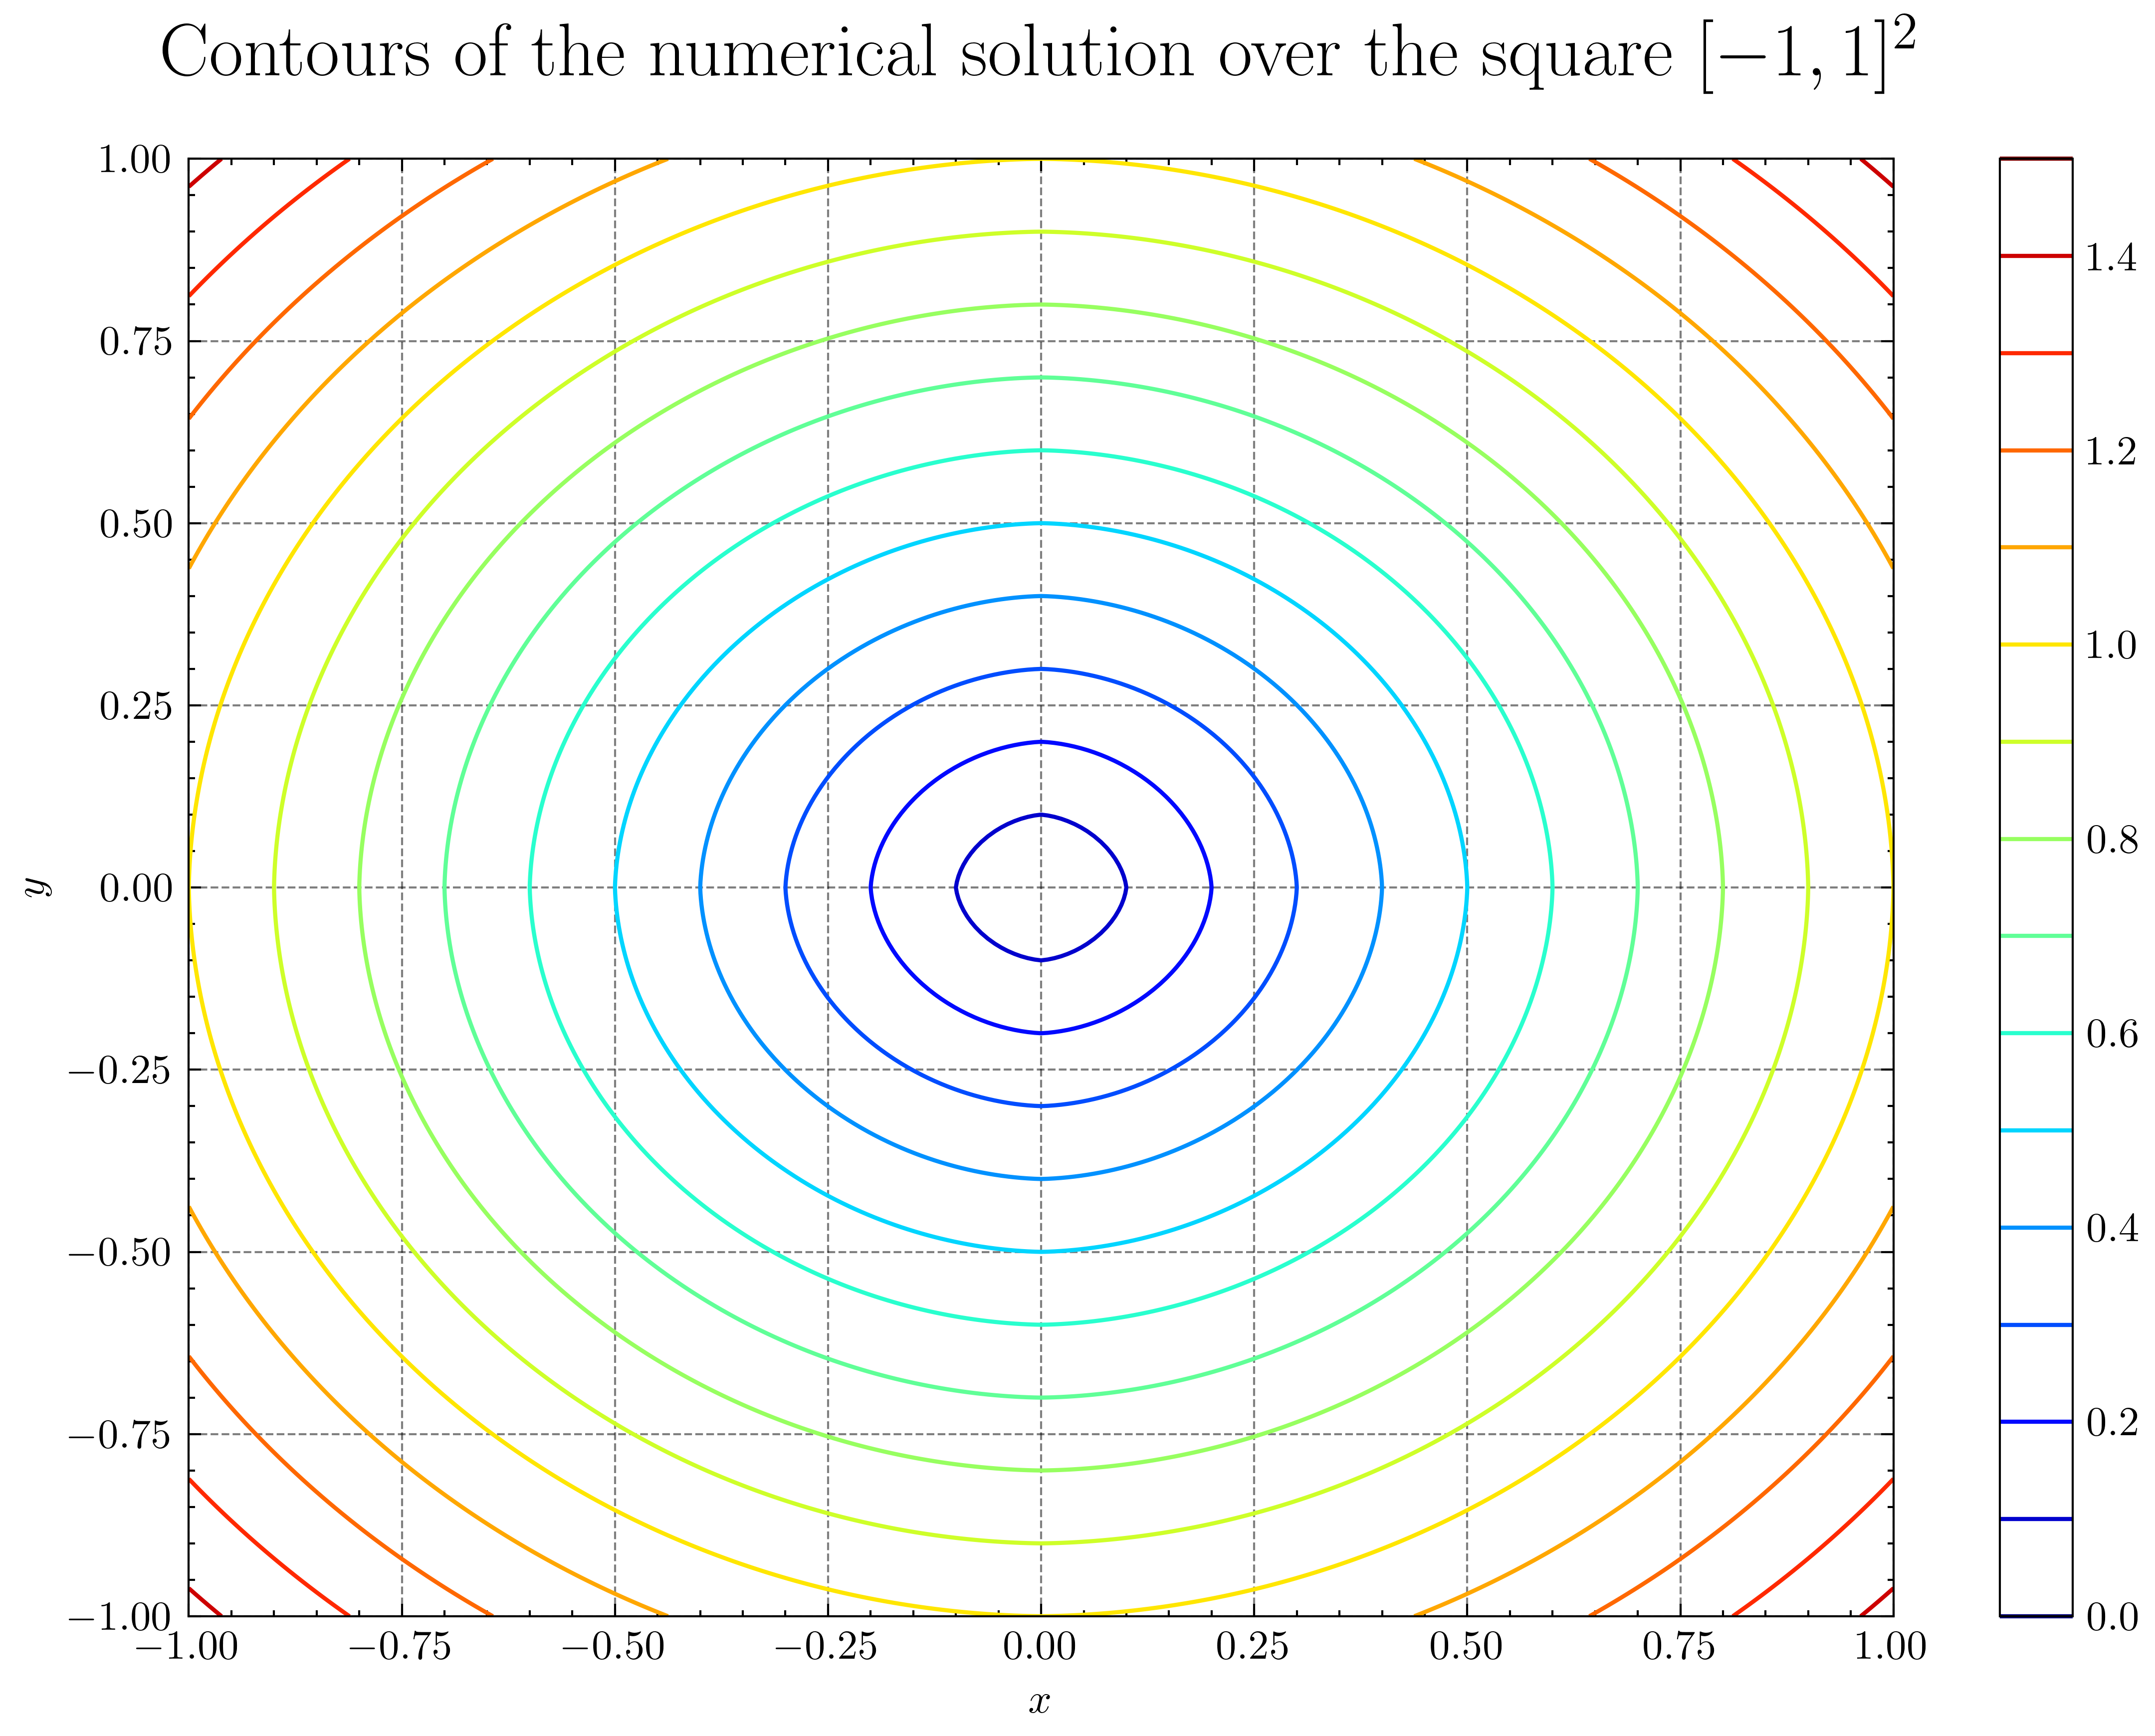
\includegraphics[width=\linewidth]{plots/contour_plot_2D_distance.png}
        \caption{Contour plot of the numerical solution to (\ref{cone_bvp}).}
        \label{fig:contour-distance}
    \end{minipage}
    \hfill
    \begin{minipage}{0.48\linewidth}
        \centering
        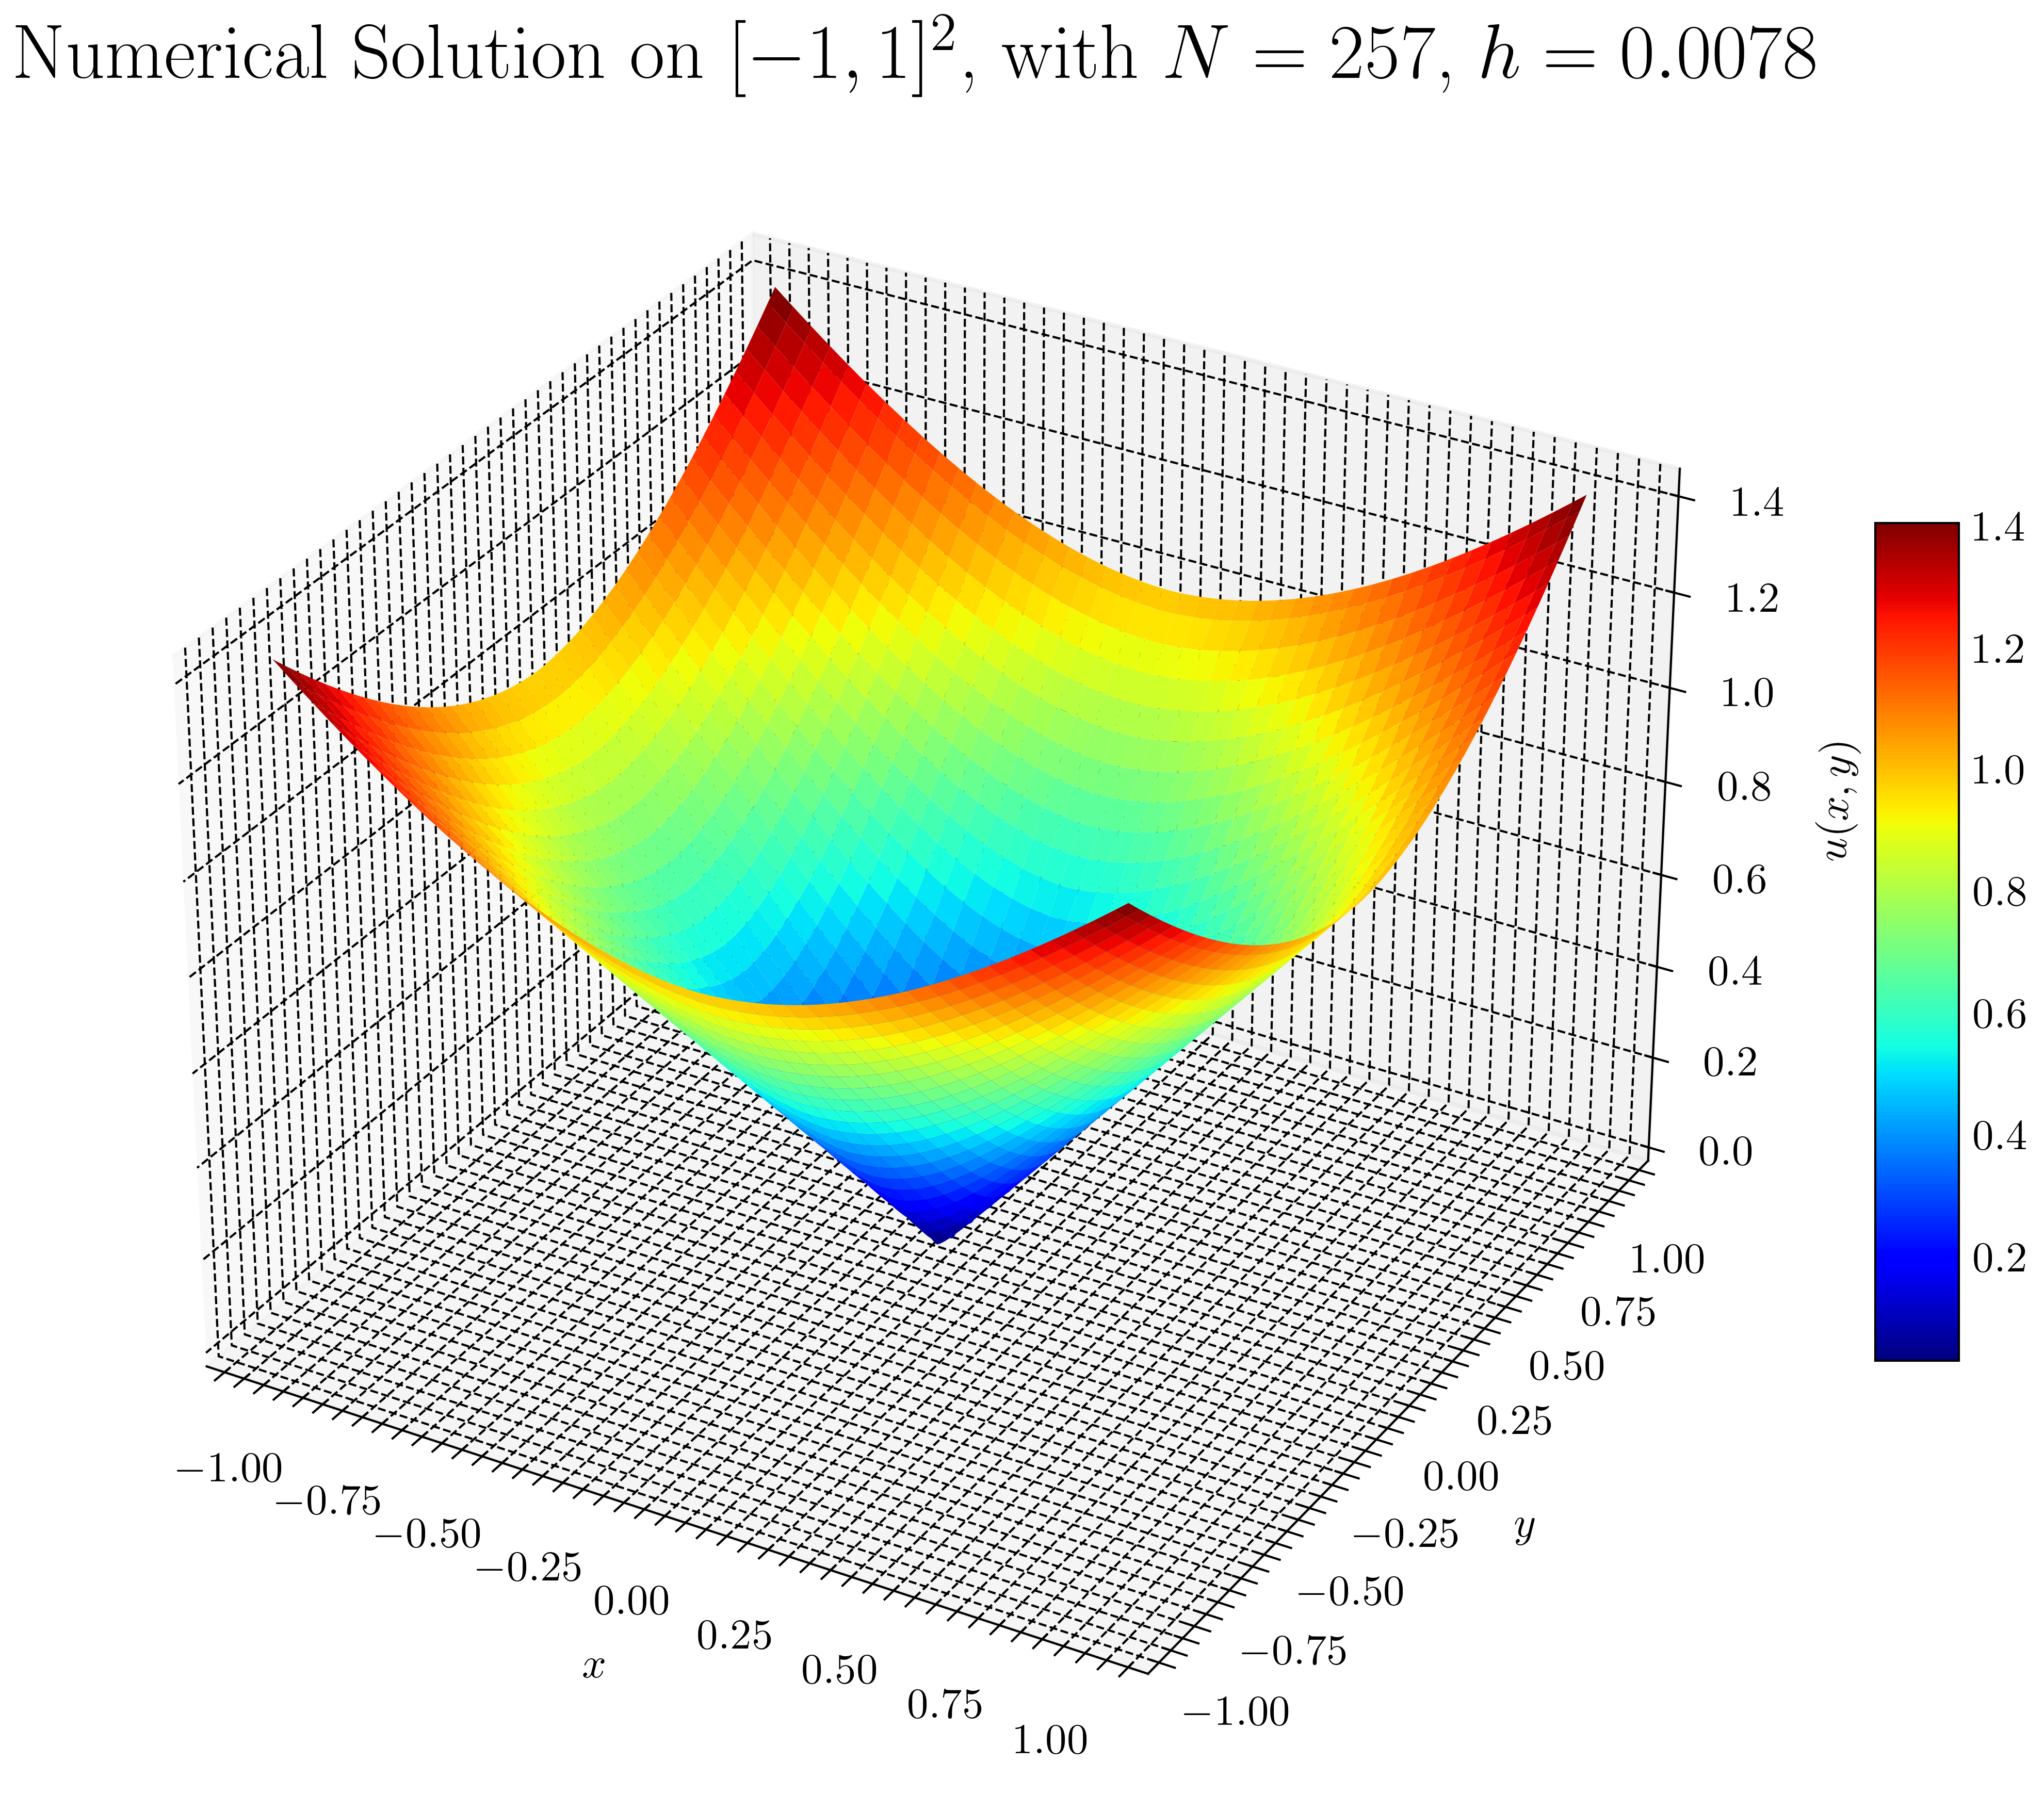
\includegraphics[width=\linewidth]{plots/solution_3d_surface.png}
        \caption{3D surface of the numerical solution.}
        \label{fig:3d-surface}
    \end{minipage}
\end{figure}

\FloatBarrier

\noindent Figure (\ref{fig:contour-distance}) shows the contour plots of the numerical solution. Note that since the analytical solution is $u(x,y)=\sqrt{x^2+y^2}$, we would expect in theory to have perfectly round circles. However, this remains a numerical approximation, explaining why we are seeing "oval" forms rather than perfect circles. If one were to decrease the step size $h$ (i.e. increase $N$), these ovals would eventually look more and more like perfectly round circles.
Figure (\ref{fig:3d-surface}) confirms as well that the numerical solution is somewhat close the cone we would expect. \\

\subsubsection{Convergence}
Finally, we can analyze the convergence of the fast sweeping method for the BVP (\ref{cone_bvp}). The plot below was obtained was solving numerically the BVP, using $N\in\{201, 221,241,\dots,701\}$, converting to step sizes $h=\frac{N-1}{b-a}$. For every of these values, the numerical solutions is compared to the analytic solution. Specifically, the error is computed with the $\|\cdot\|_\infty$ norm over the square $[-1,1]^2$. \\
On figure (\ref{fig:error_distance}) below, we see that the accuracy of the fast sweeping method indeed seems to be of order $O(|h\log h|)$ in this case.


\begin{figure}[h]
  \centering
  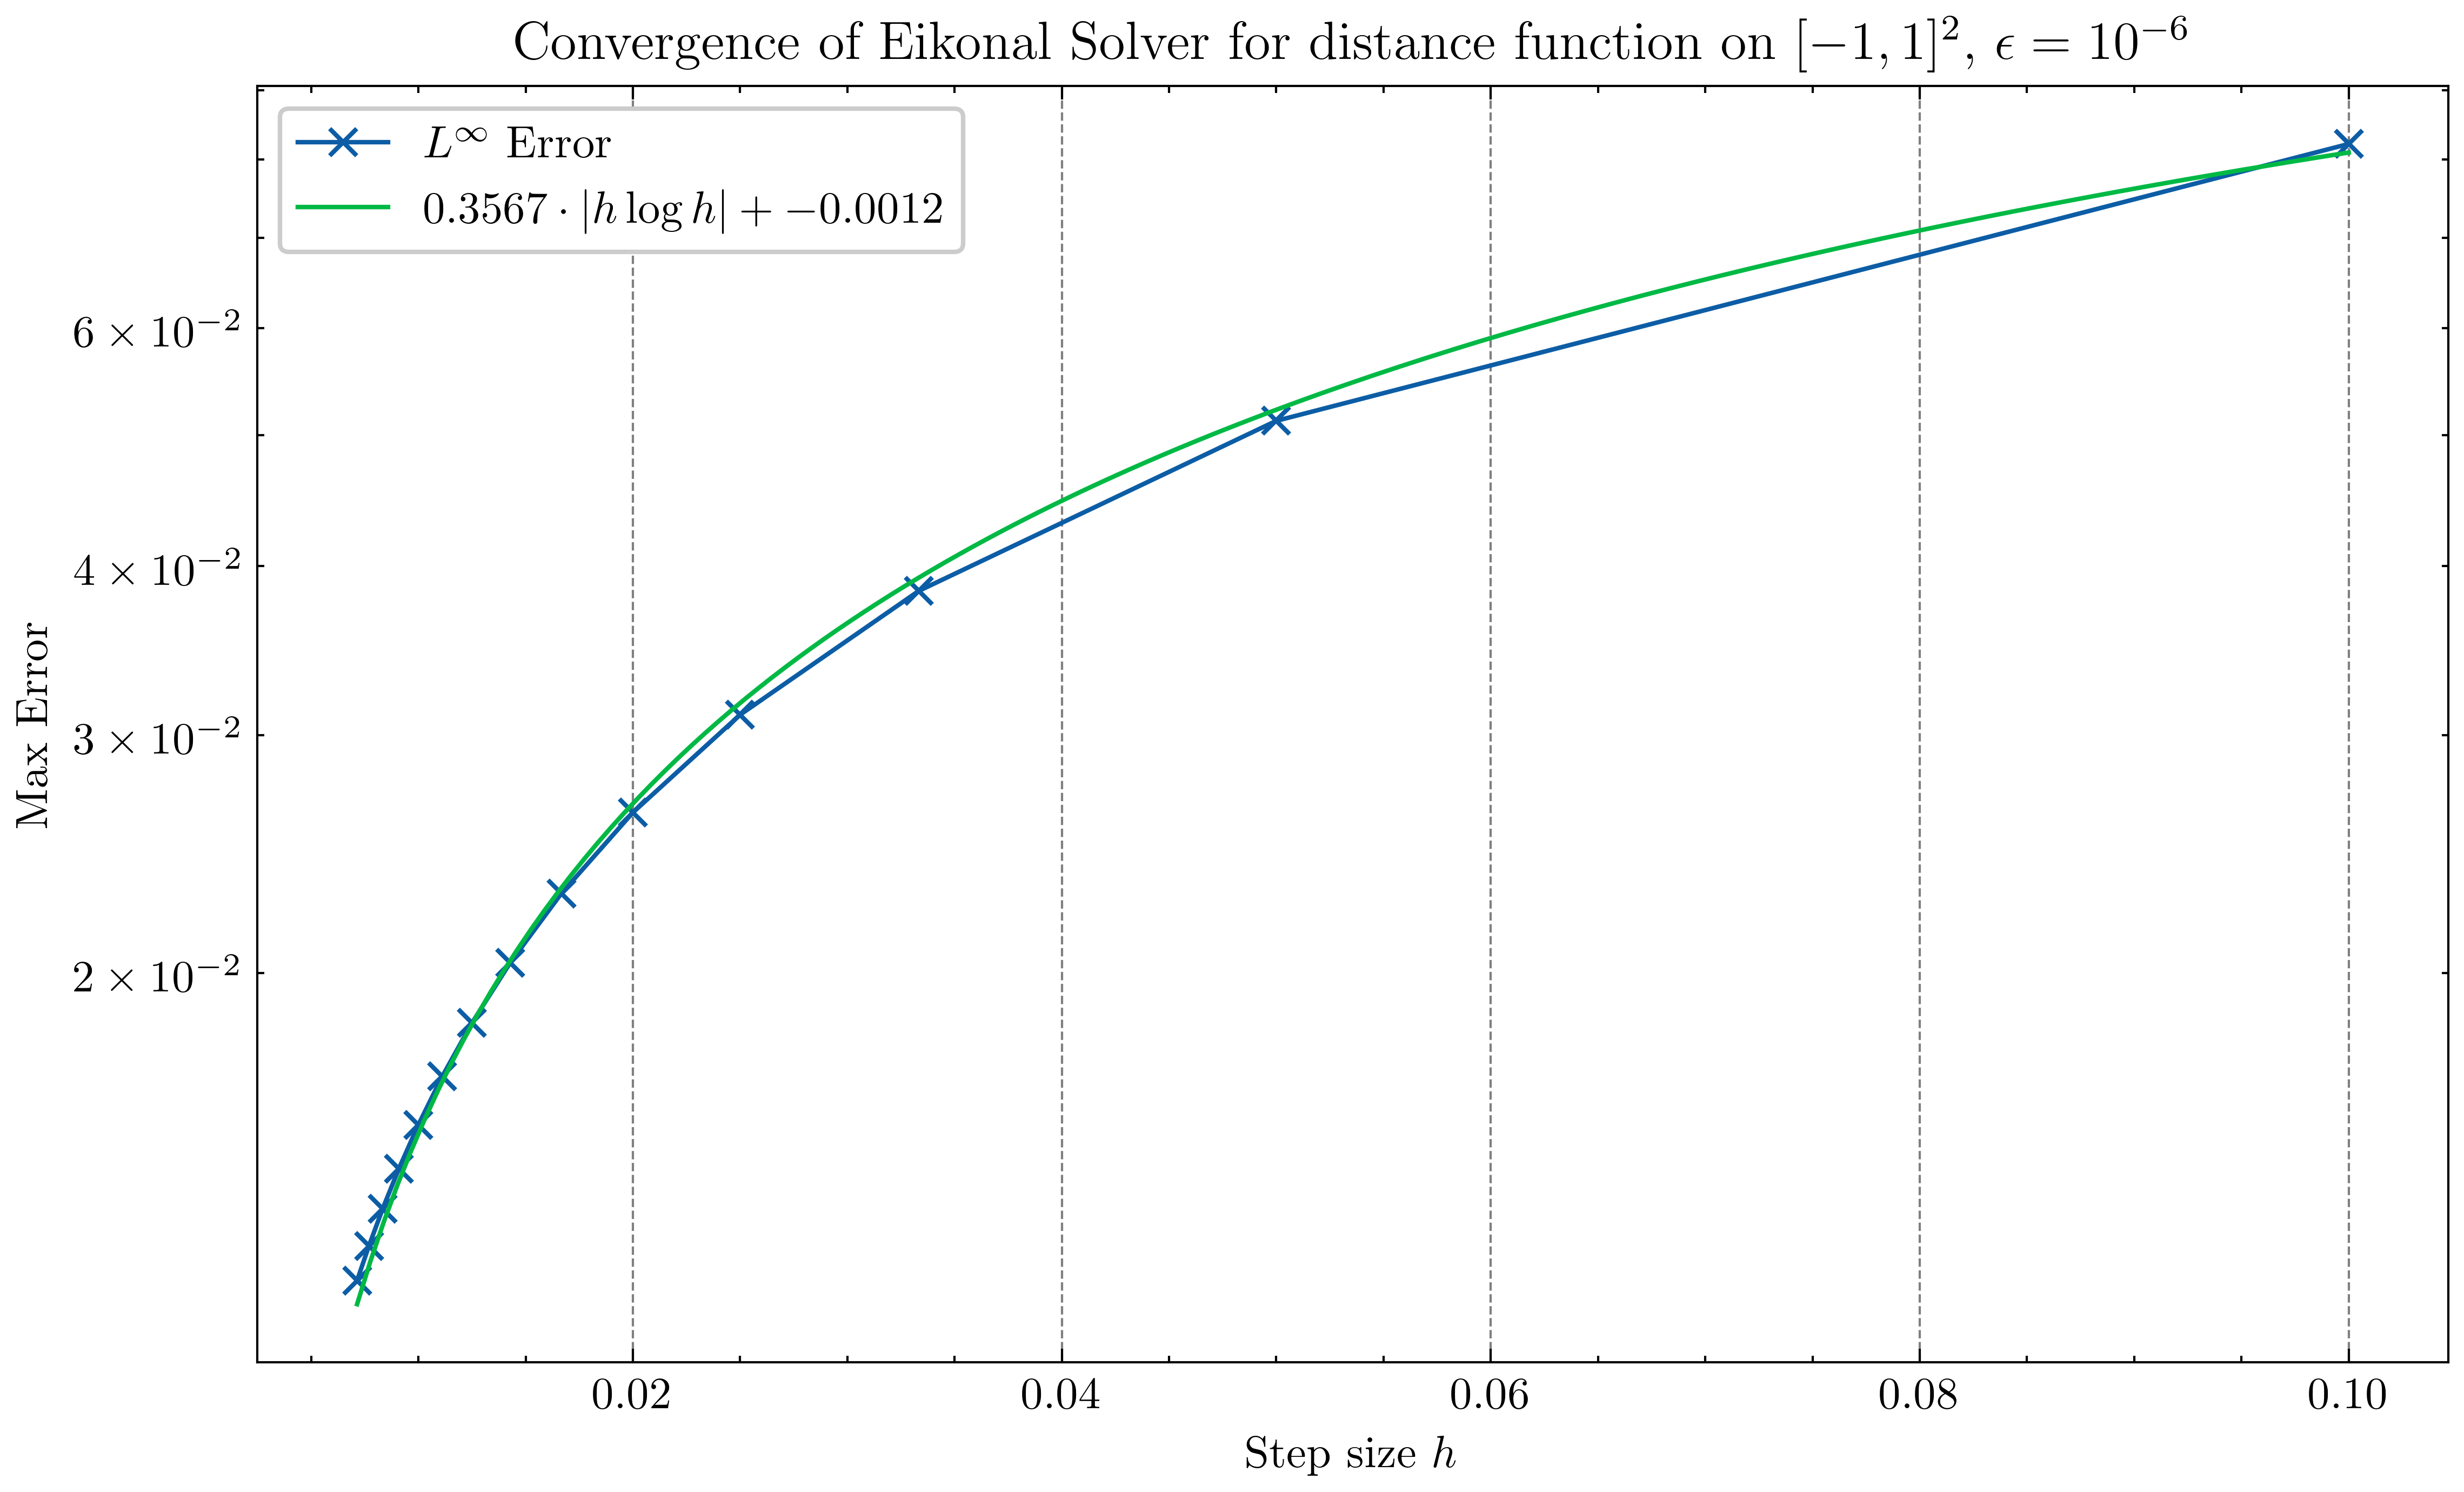
\includegraphics[width=0.7\linewidth]{plots/convergence2d_step_size.png}
  \caption{Accuracy of the fast-sweeping method for the distance function to the origin}
  \label{fig:error_distance}
\end{figure}

\subsection{Distance functions in 2D with several boundary points}
The example in the previous subsection was only considering one boundary value at the origin of the domain, i.e. the set $\Gamma$ was simply $\Gamma=\{(0,0)\}$. We can introduce several other boundary points, and the solution $u$ picked up by the fast sweeping-method will give at any point $(x,y)$ the distance to the closest point $\gamma\in\Gamma$, as we showed in section (\ref{section_on_distance}). Indeed consider the case below, where we chose 5 points at random on $[-1,1]^2$, and set these points to be 0 in the domain. Our Eikonal solver then converges to the numerical solution $u(x,y)$ whose contours and 3D surface are given by figures (\ref{fig:contour5}) and (\ref{fig:surface5}) respectively. \\
It is easy to see on both the contour plots and on the 3D surface that the solution is non-differentiable on some lines inside the domain. In particular, the points on these lines are the ones lying at the same distance to at least 2 boundary points in $\Gamma$. In other words, the problem (\ref{min-problem}) does not have a unique minimizer for these sets of points.

\vspace{5pt}

\begin{figure}[h]
  \centering
  \begin{minipage}{0.45\textwidth}
    \centering
    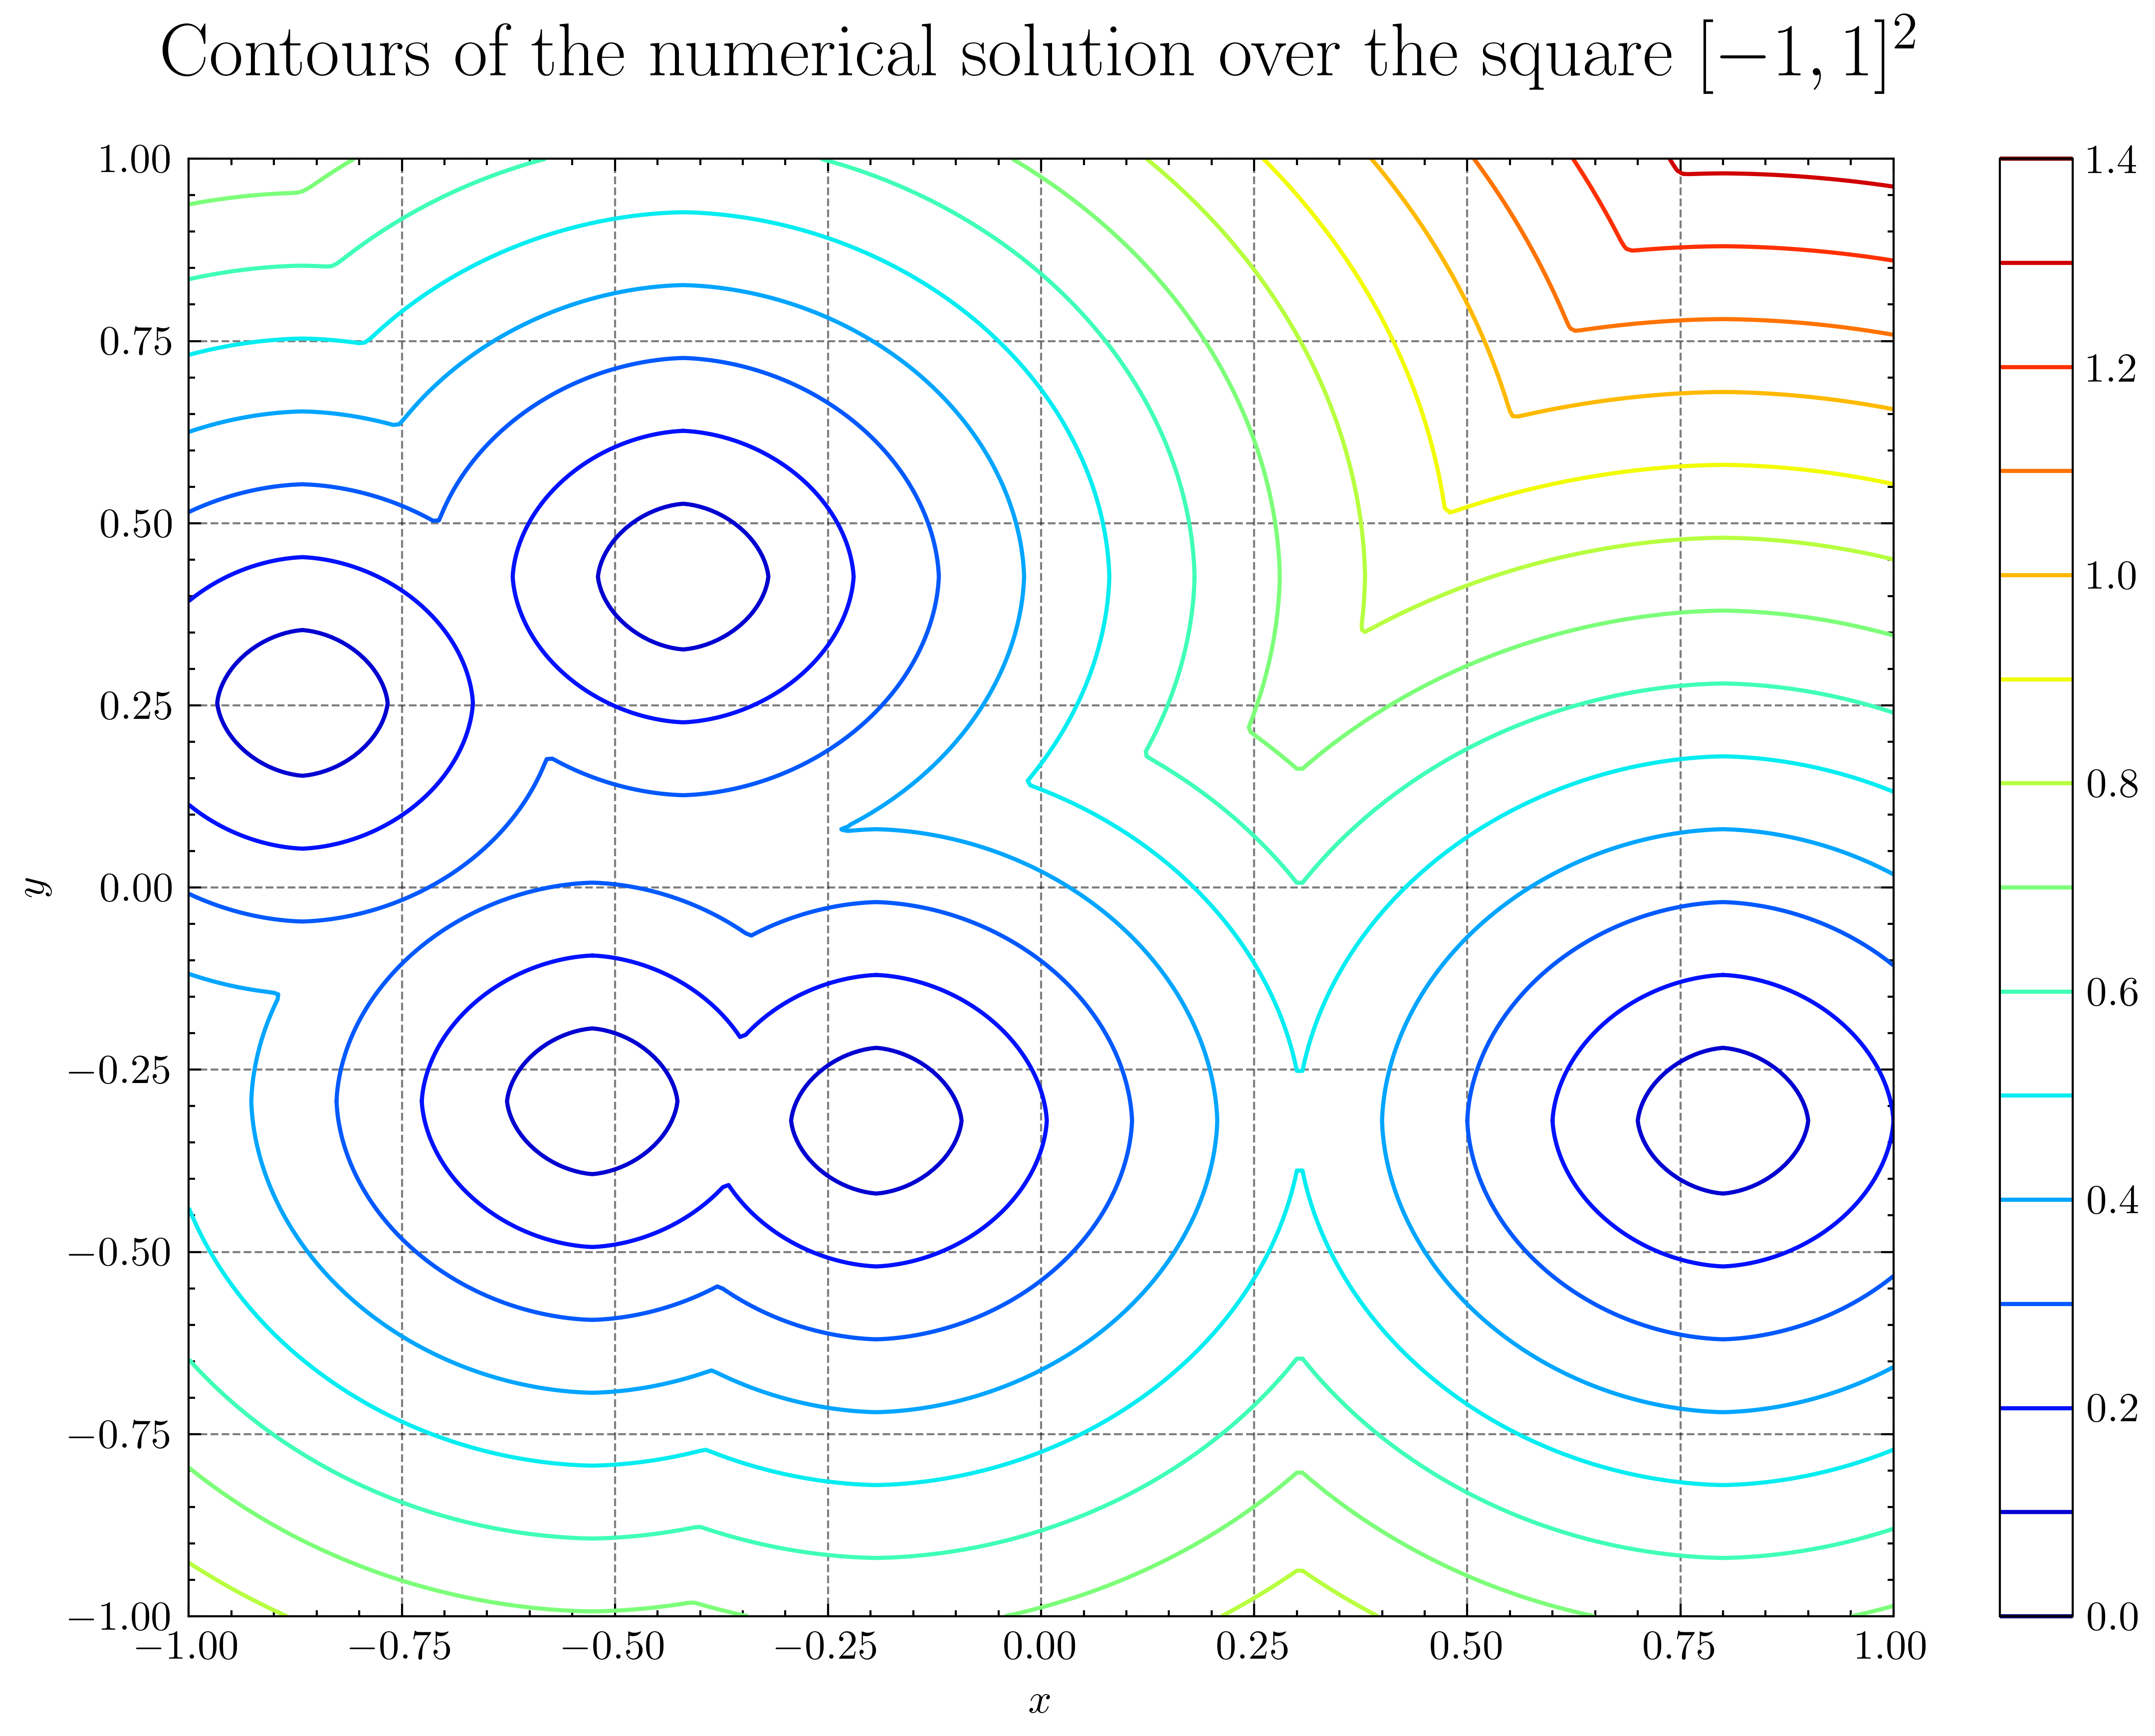
\includegraphics[width=\linewidth]{plots/contour_plot_random5.png}
    \caption{Contours of numerical solution ($|\Gamma|=5$)}
    \label{fig:contour5}
  \end{minipage}
  \hfill
  \begin{minipage}{0.45\textwidth}
    \centering
    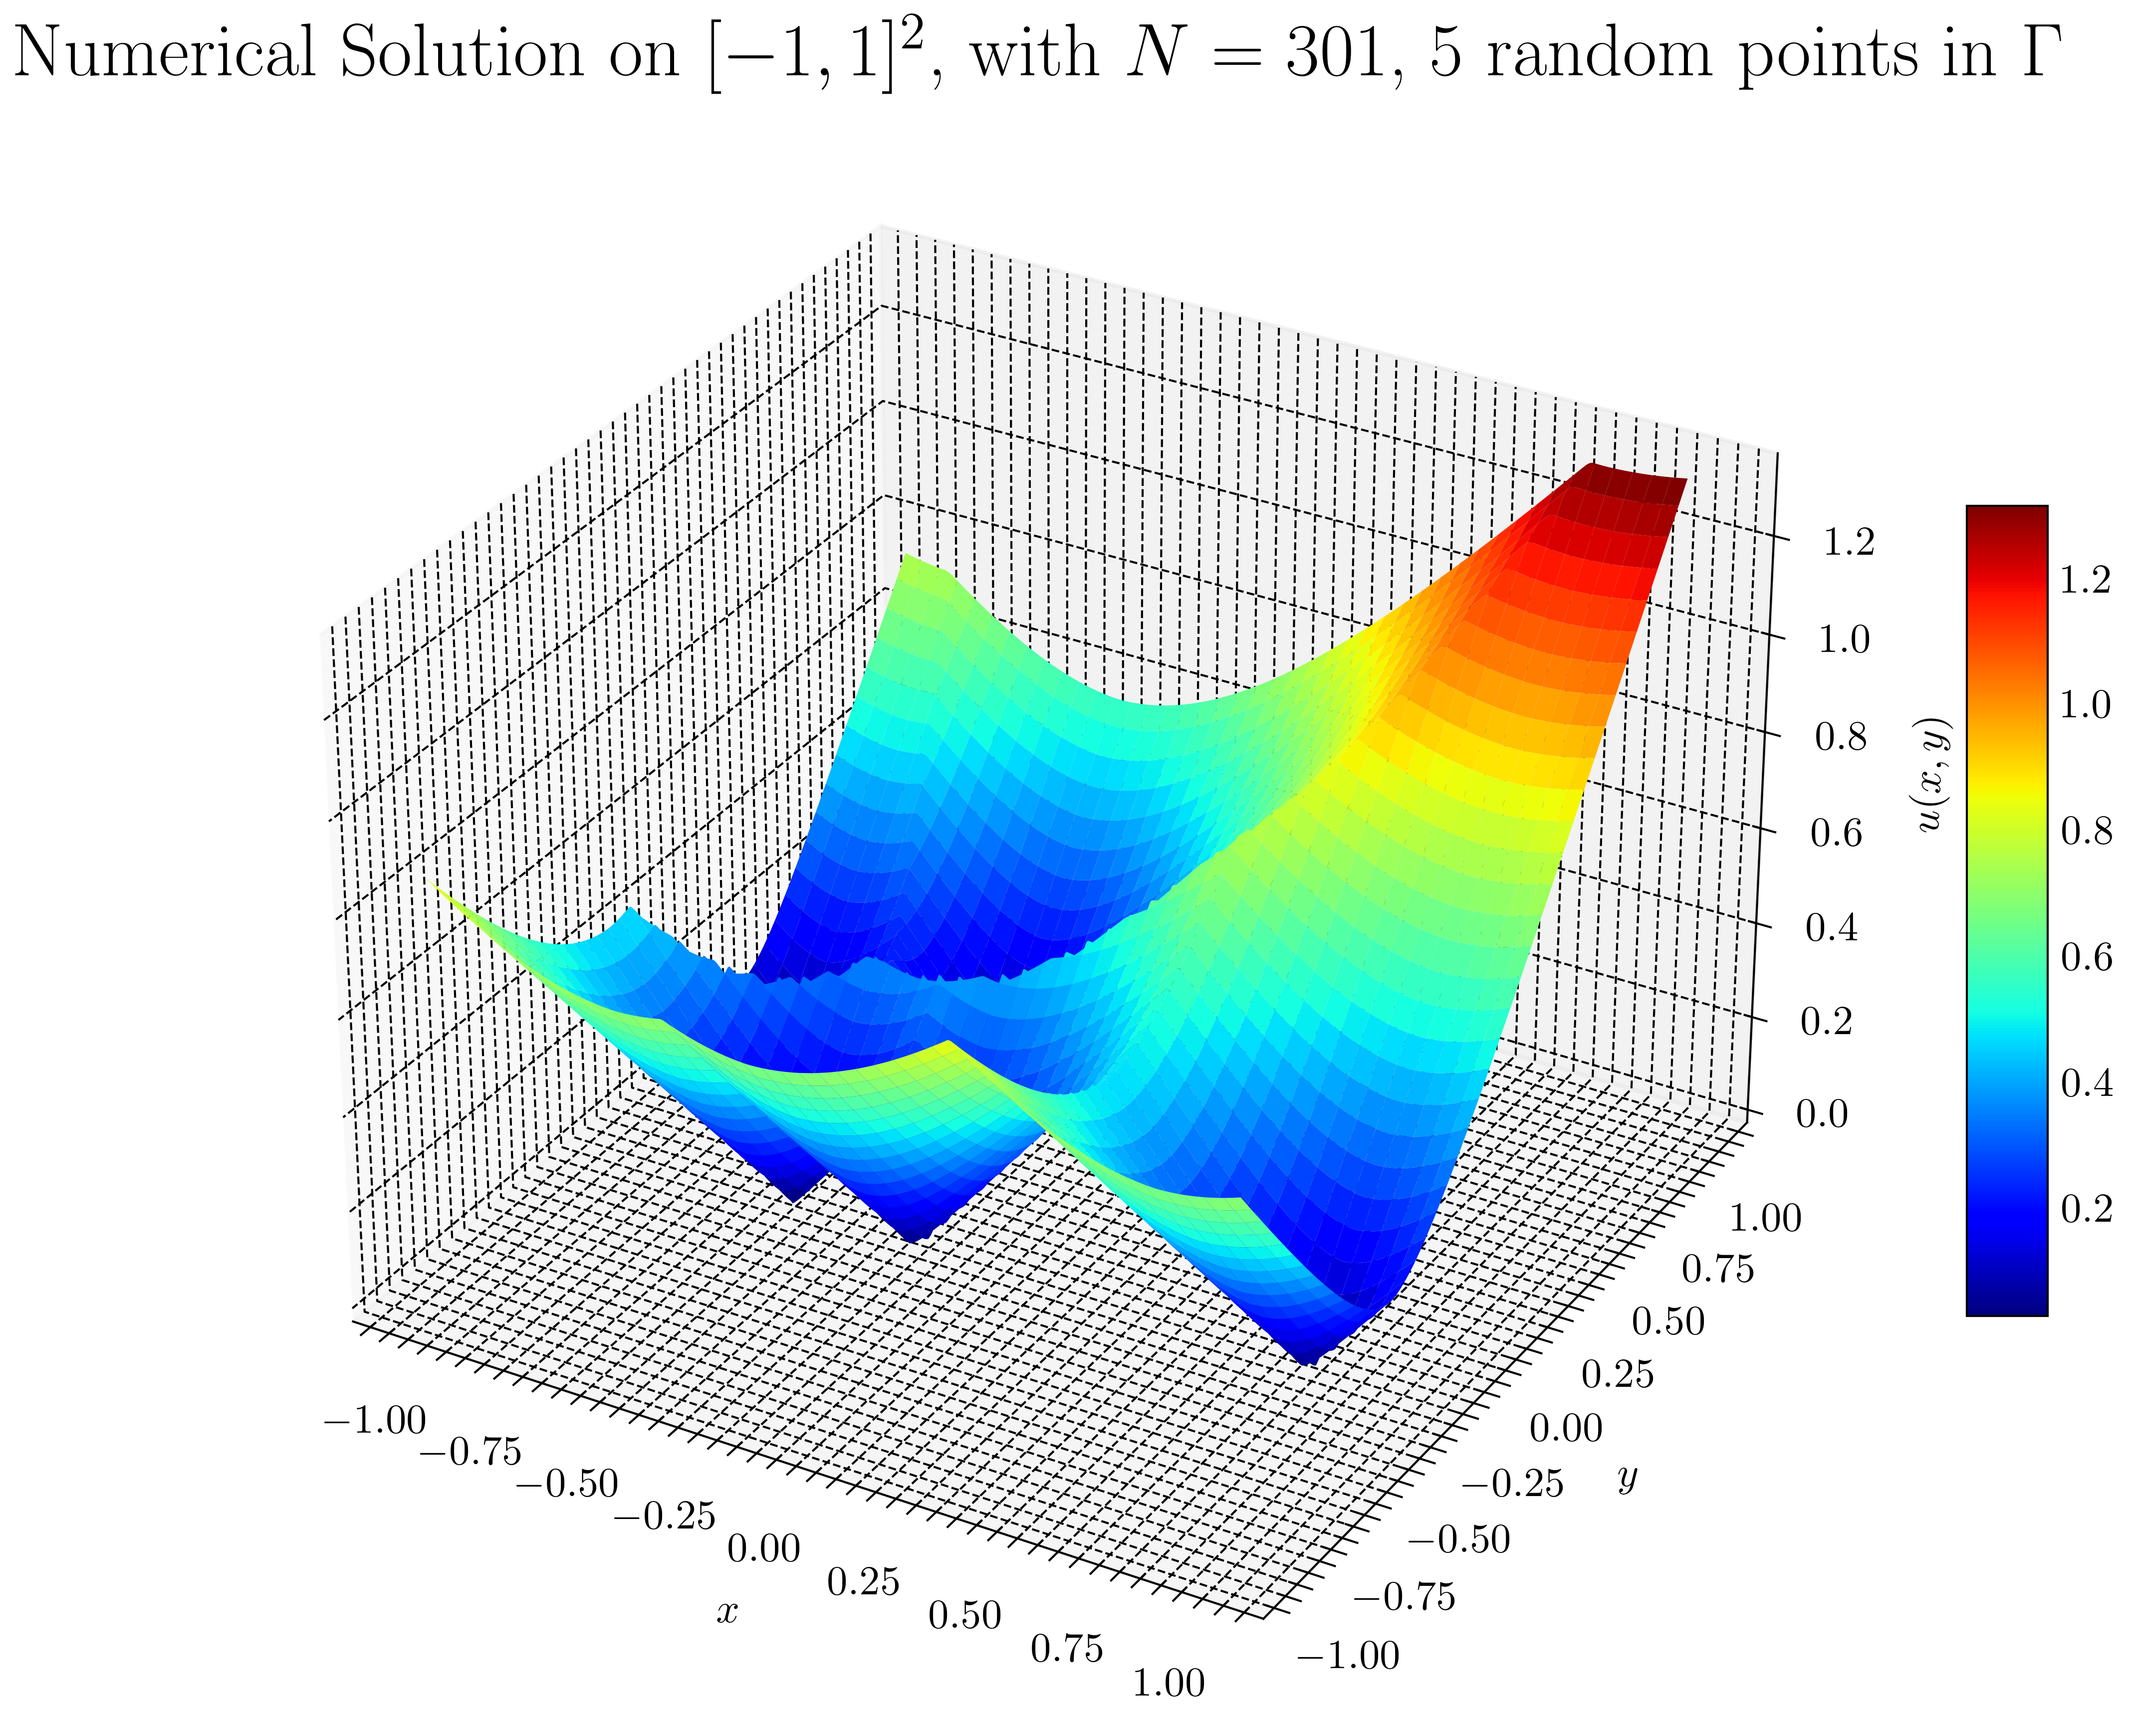
\includegraphics[width=\linewidth]{plots/solution_3d_surface_random5.png}
    \caption{3D surface of the solution ($|\Gamma$|=5)}
    \label{fig:surface5}
  \end{minipage}
\end{figure}

\FloatBarrier

\noindent Finally, we look at another case where we introduce several more boundary points in $\Gamma$. In the example below, we sampled uniformly at random 30 points in $[-1,1]^2$ and set these points to have value 0. Figure (\ref{fig:heatmap30random}) represents a heatmap of the solution. The regions where the solution is non-differentiable are easily seen.

\begin{figure}[h!]
  \centering
  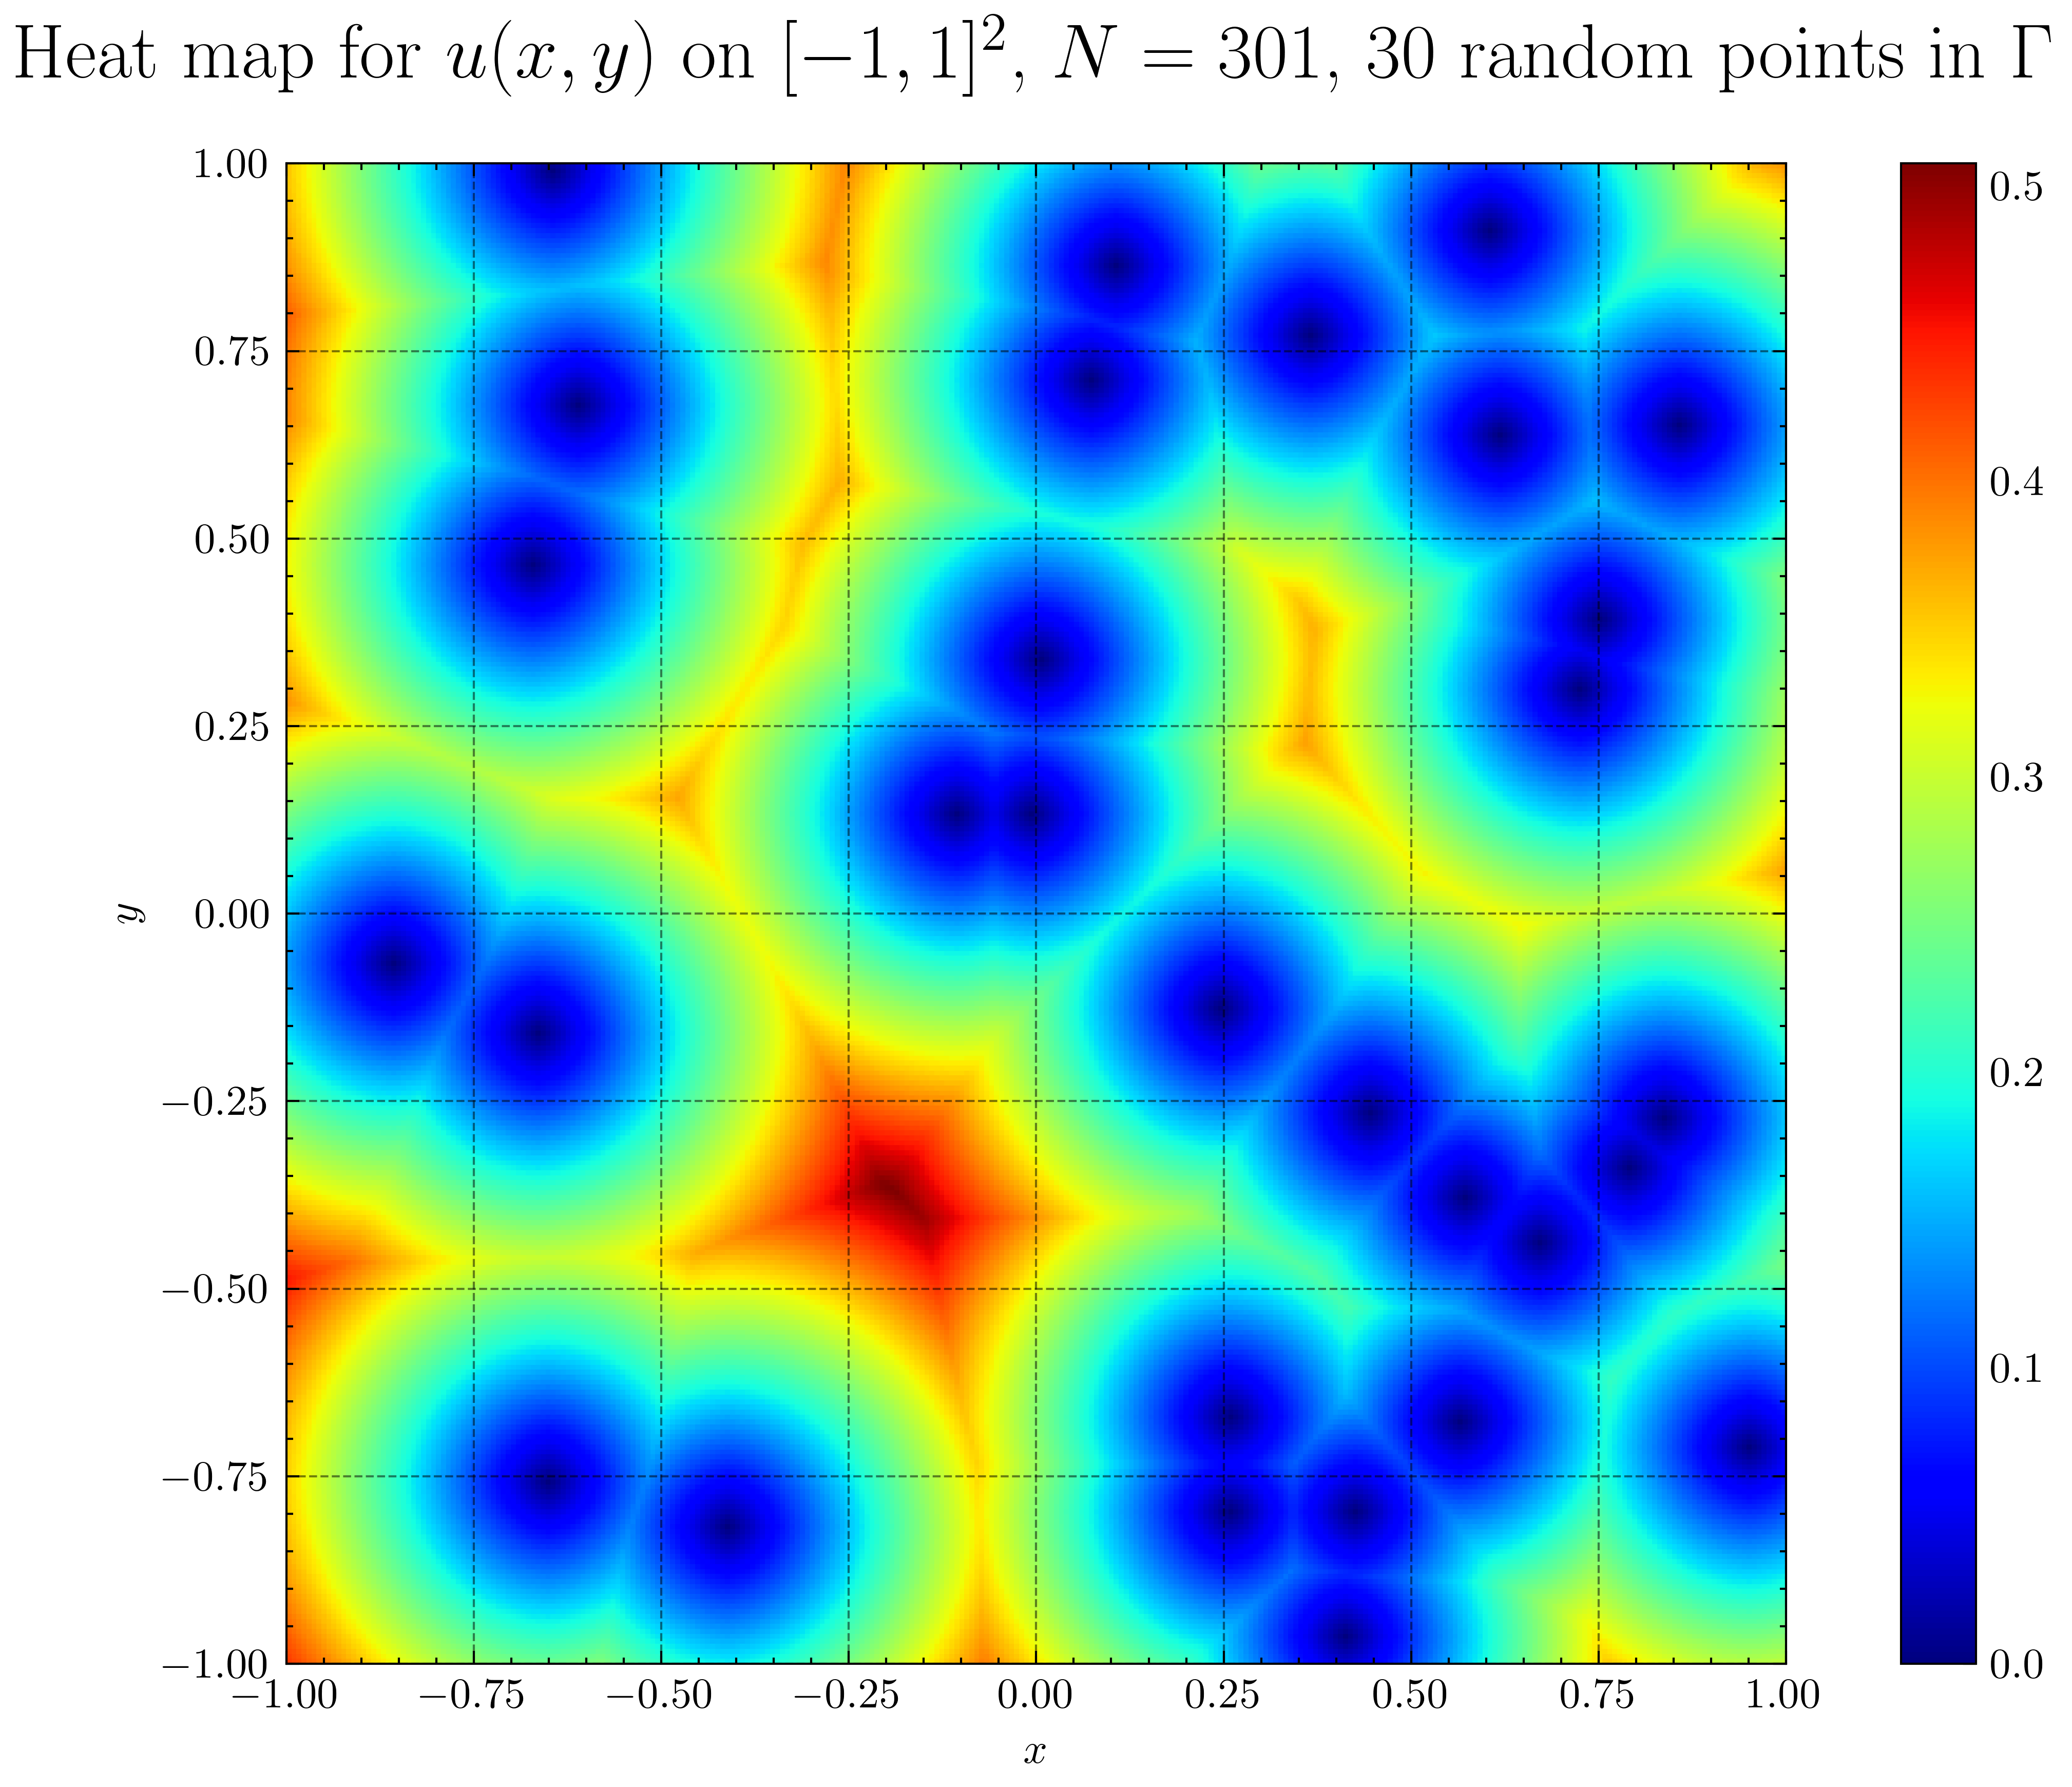
\includegraphics[width=0.5\textwidth]{plots/heatmap_random30.png}
  \caption{Distance function in 2D for $|\Gamma|=30$ (random boundary points)}
  \label{fig:heatmap30random}
\end{figure}

\newpage

\subsection{General Eikonal equations}
In this subsection, we now are interested at problems of the form of (\ref{original-eikonal}) where $f(x,y)\not\equiv 1$ on the domain. Conveniently, we will also rewrite $f(x,y)=\frac{1}{F(x,y)}$, where $F(x,y)$ can now be thought of as a velocity over the domain, as argued in the derivation in the wave (or front) propagation context. As a result, the solution $u(x,y)$ does not give the distance to the boundary anymore, but rather the "cost" of the travel from $(x,y)$ to $\Gamma$.
We test our solver for the problem.

\begin{equation}
\label{arctan_equation}
    \begin{cases}
        |\nabla u(x,y)|=\frac{1}{1+0.5(x^2+y^2)} , \quad(x,y) \in [-2,2]^2 \\
        u(0,0)= 0
    \end{cases}
\end{equation} \\

\noindent One can check that $u(x,y)=\sqrt{2}\arctan\Big[\sqrt{\frac{x^2+y^2}{2}}\Big]$ solves (\ref{arctan_equation}). We use this reference to test our solver with the following parameters : $N=801$ on the discretized domain $[-2,2]^2$ which gives the step size $h=0.005$, with convergence criterion $\epsilon=10^{-6}$. The contours and surface of the numerical solution are displayed below on figures (\ref{fig:contour_arctan}) and (\ref{fig:surface_arctan}). \\

\begin{figure}[h]
  \centering
  \begin{minipage}{0.45\textwidth}
    \centering
    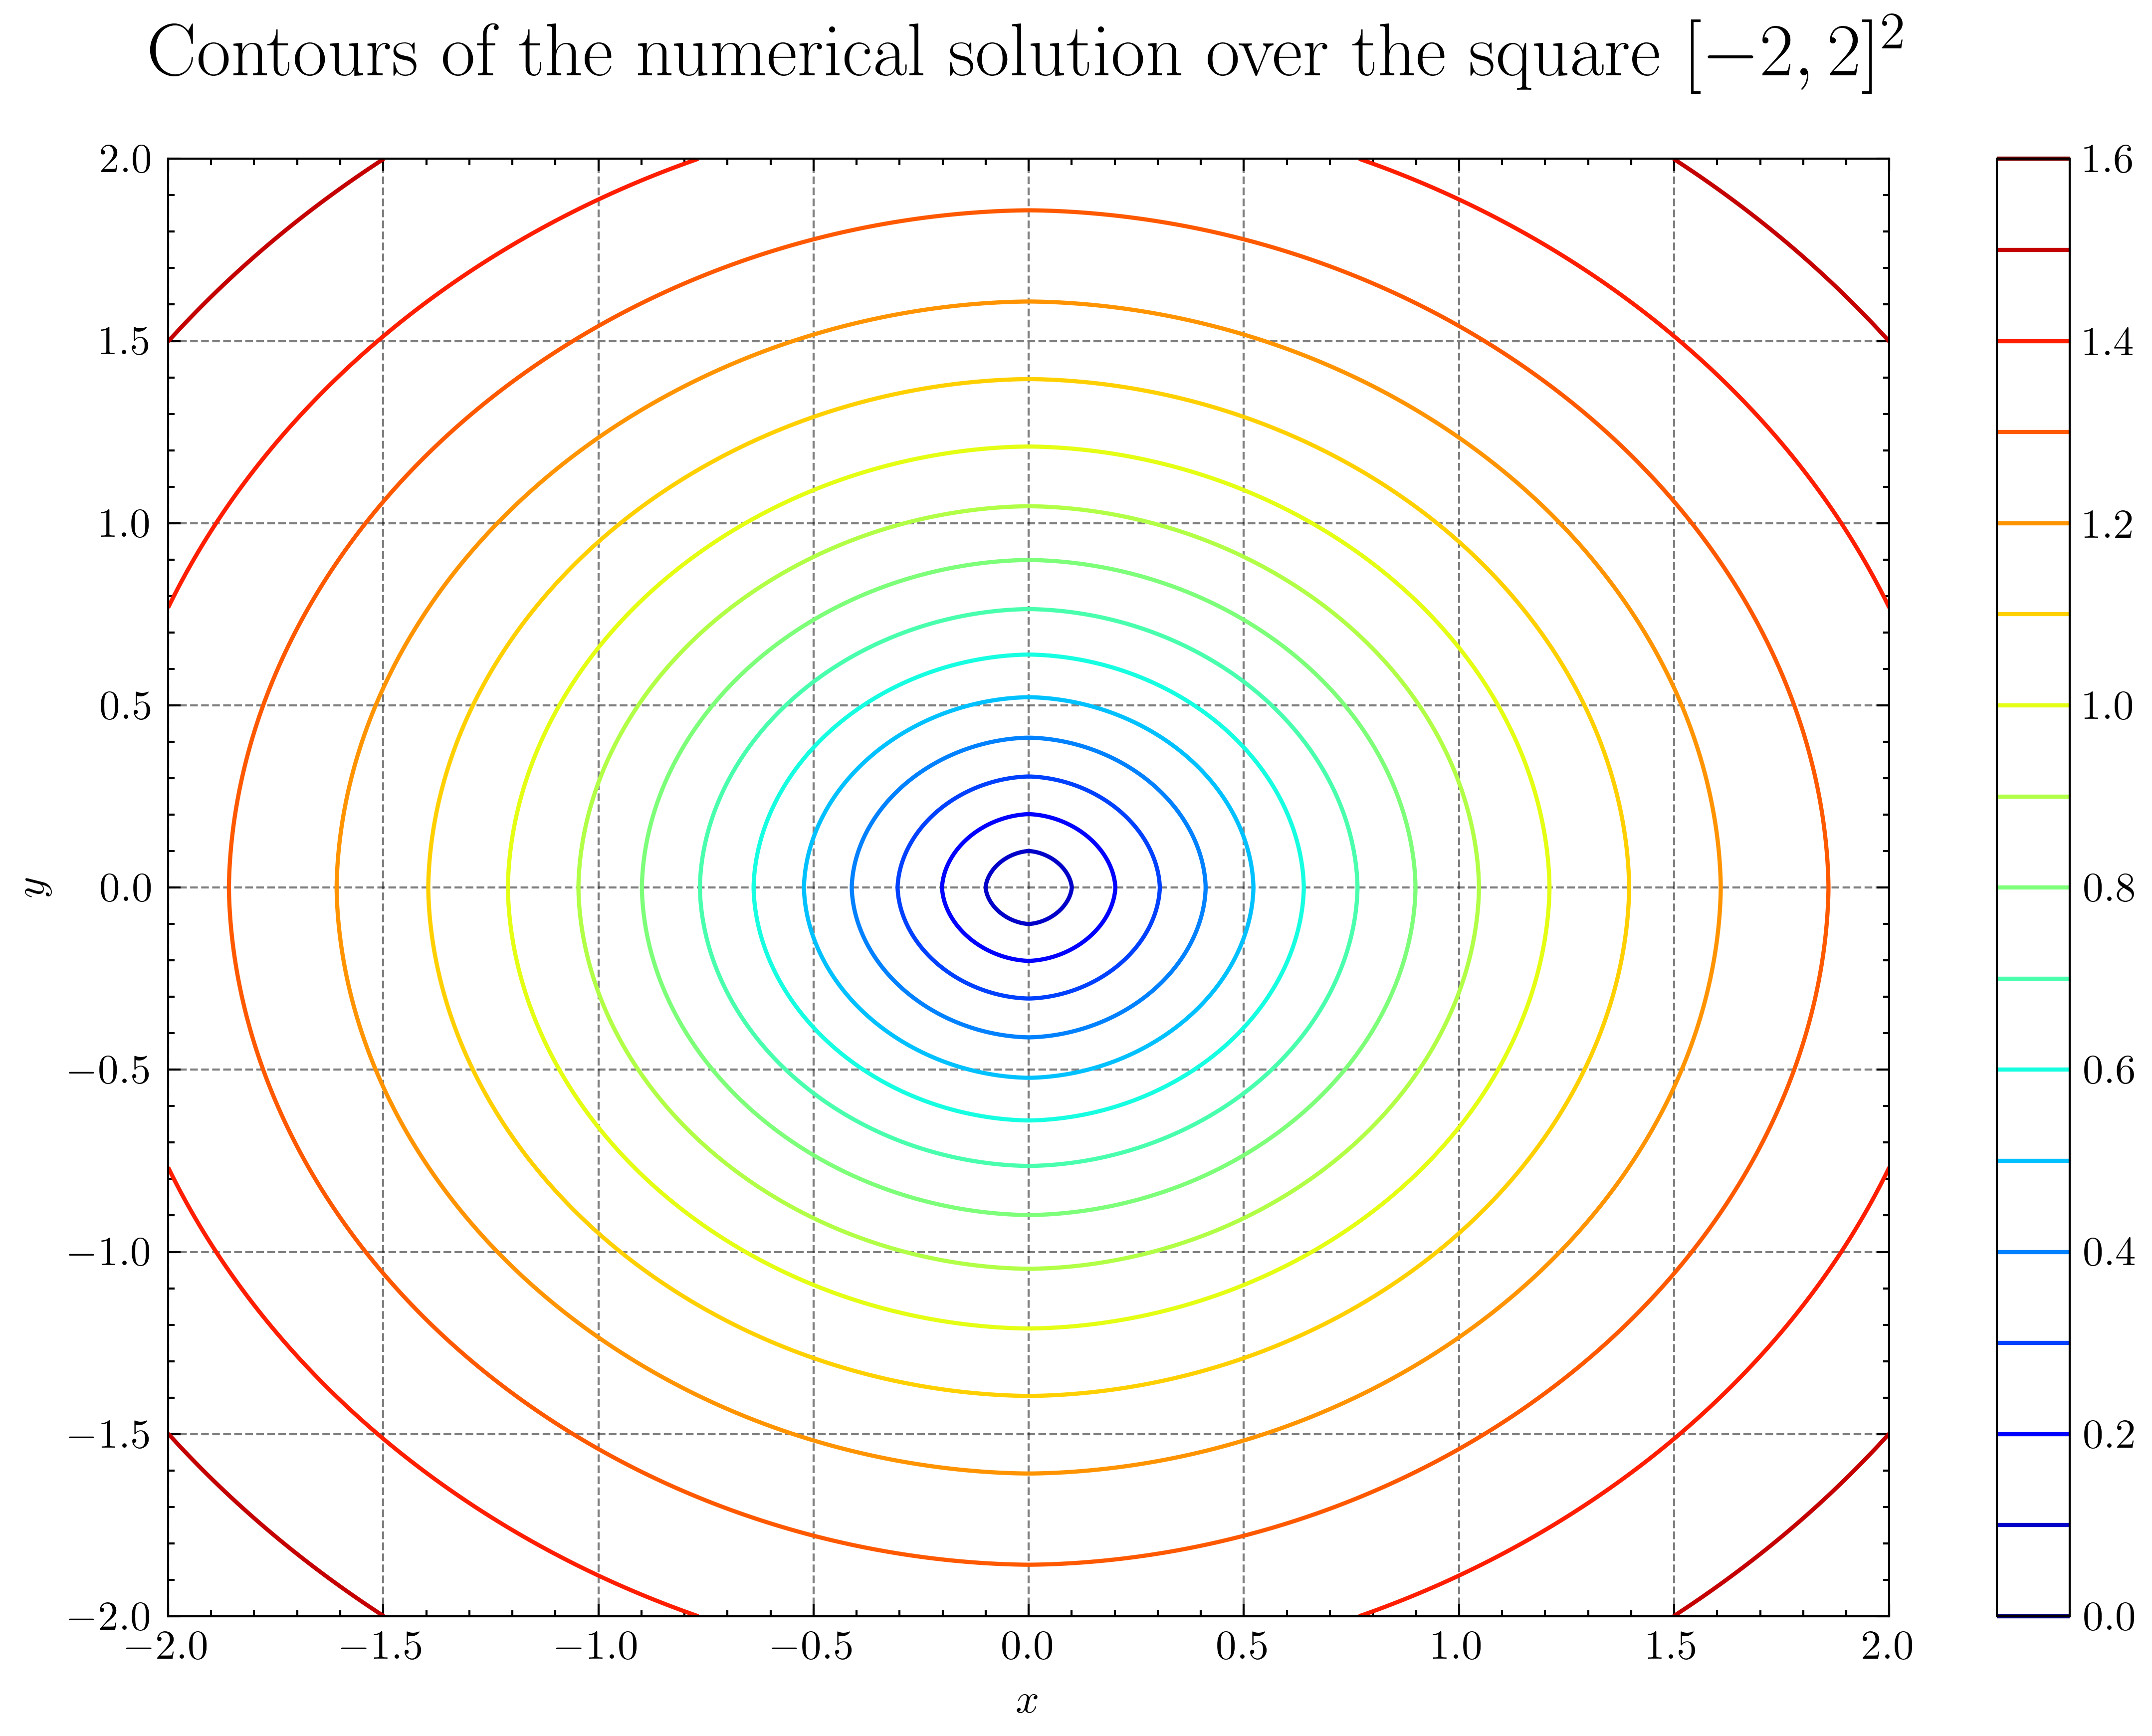
\includegraphics[width=\linewidth]{plots/contour_plot_arctan.png}
    \caption{Contours of numerical solution where $F(x,y)=1+0.5(x^2+y^2)$}
    \label{fig:contour_arctan}
  \end{minipage}
  \hfill
  \begin{minipage}{0.45\textwidth}
    \centering
    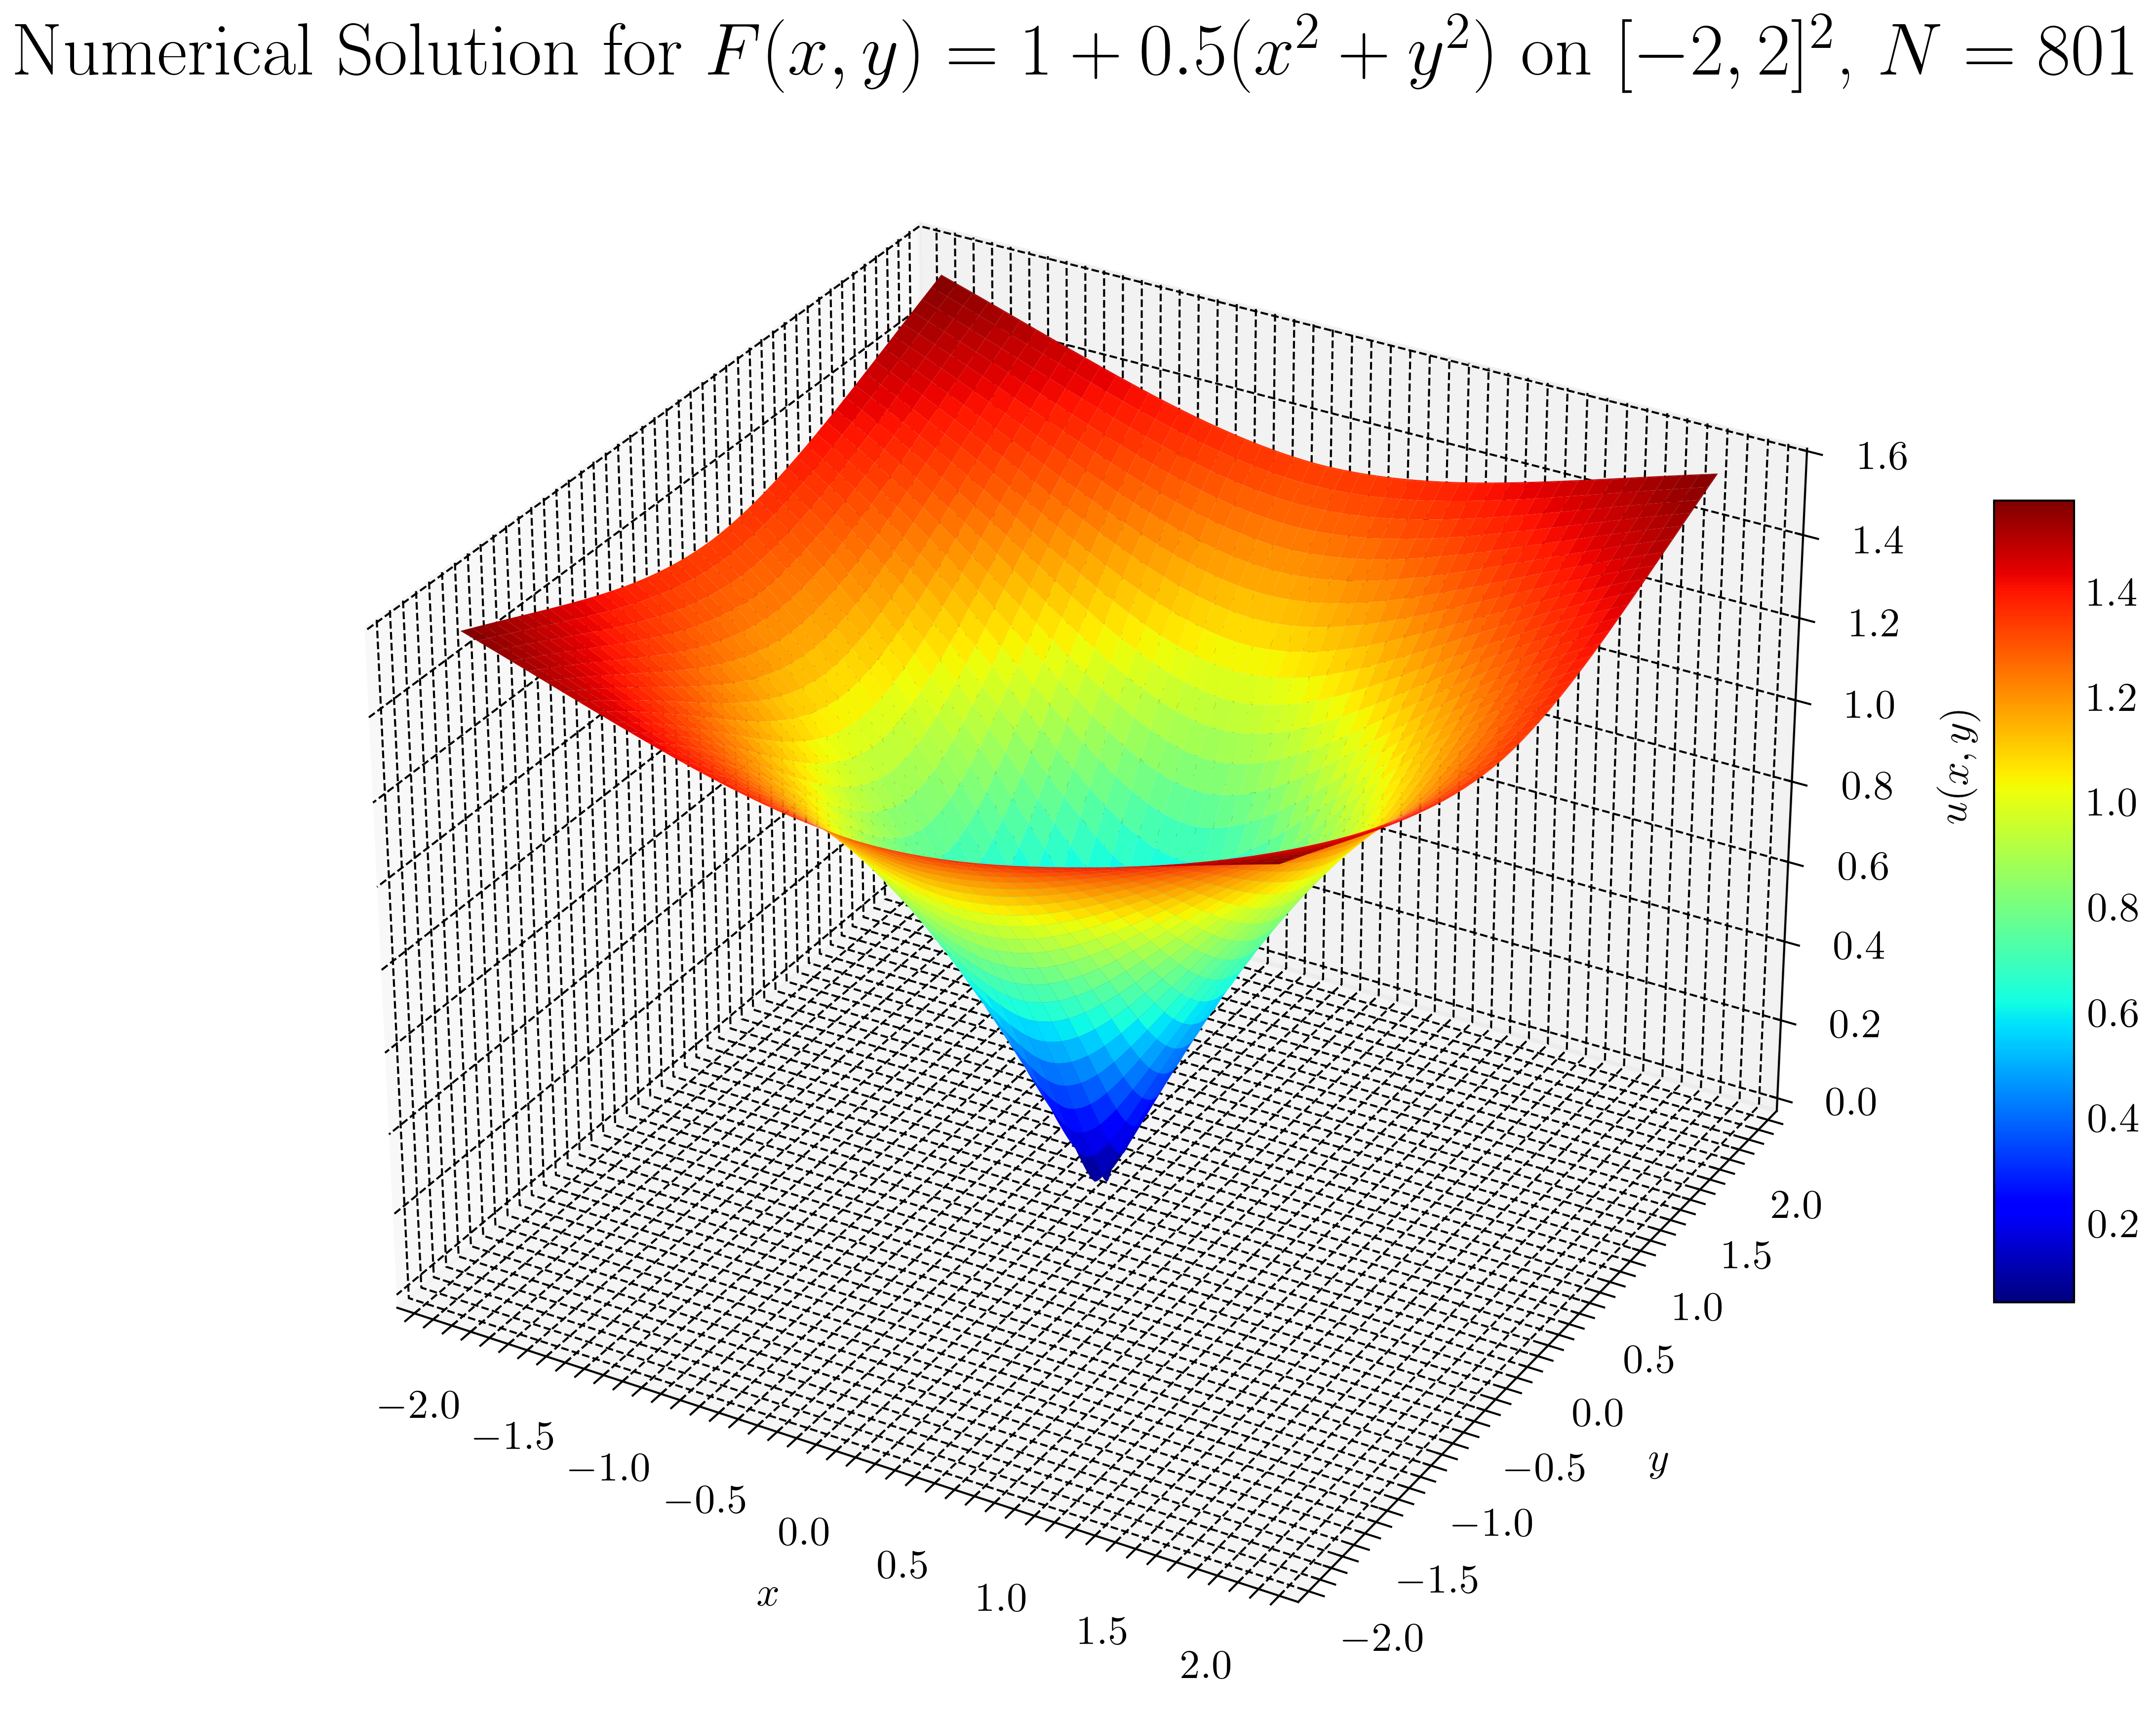
\includegraphics[width=\linewidth]{plots/solution_3d_surface_arctan.png}
    \caption{3D surface of the numerical solution}
    \label{fig:surface_arctan}
  \end{minipage}
\end{figure}

\subsubsection{Convergence}
From Zhao, we know that for the general case $1/F(x,y)\not\equiv1$, we believe that fast-sweeping method also converges to the true solution in $\mathcal{O}(h\log h)$ in this specific case. For the reference problem defined in the section above, with $N\in\{751,1001,\dots,3751\}\implies h\in\{0.0013,0.001,\dots,0.00027\}$, we get the following convergence to the true solution. To reduce the computational cost and increase the accuracy, we reduced the domain to $\Omega=[-0.5,0.5]^2$. This convergence plot took about 40 minutes to be obtained. \\
An important point is that we were at first not entirely sure that the order of accuracy would be $h\log h$ for this specific case. In particular, we were hesitating between $\sqrt{h}$ and $h\log h$. This led us to choosing quite small values for $h$ in order to increase our chance of seeing the asymptotic results to kick in. \\
We fitted two linear models : $\beta_0+\beta_1\sqrt{h}$ and $\beta_0+\beta_1h\log h$ and the $R^2$ scores for the models were respectively 0.9951 and 0.9999 reinforcing our belief that the accuracy should be of order $h\log h$
.
\begin{figure}[h]
  \centering
  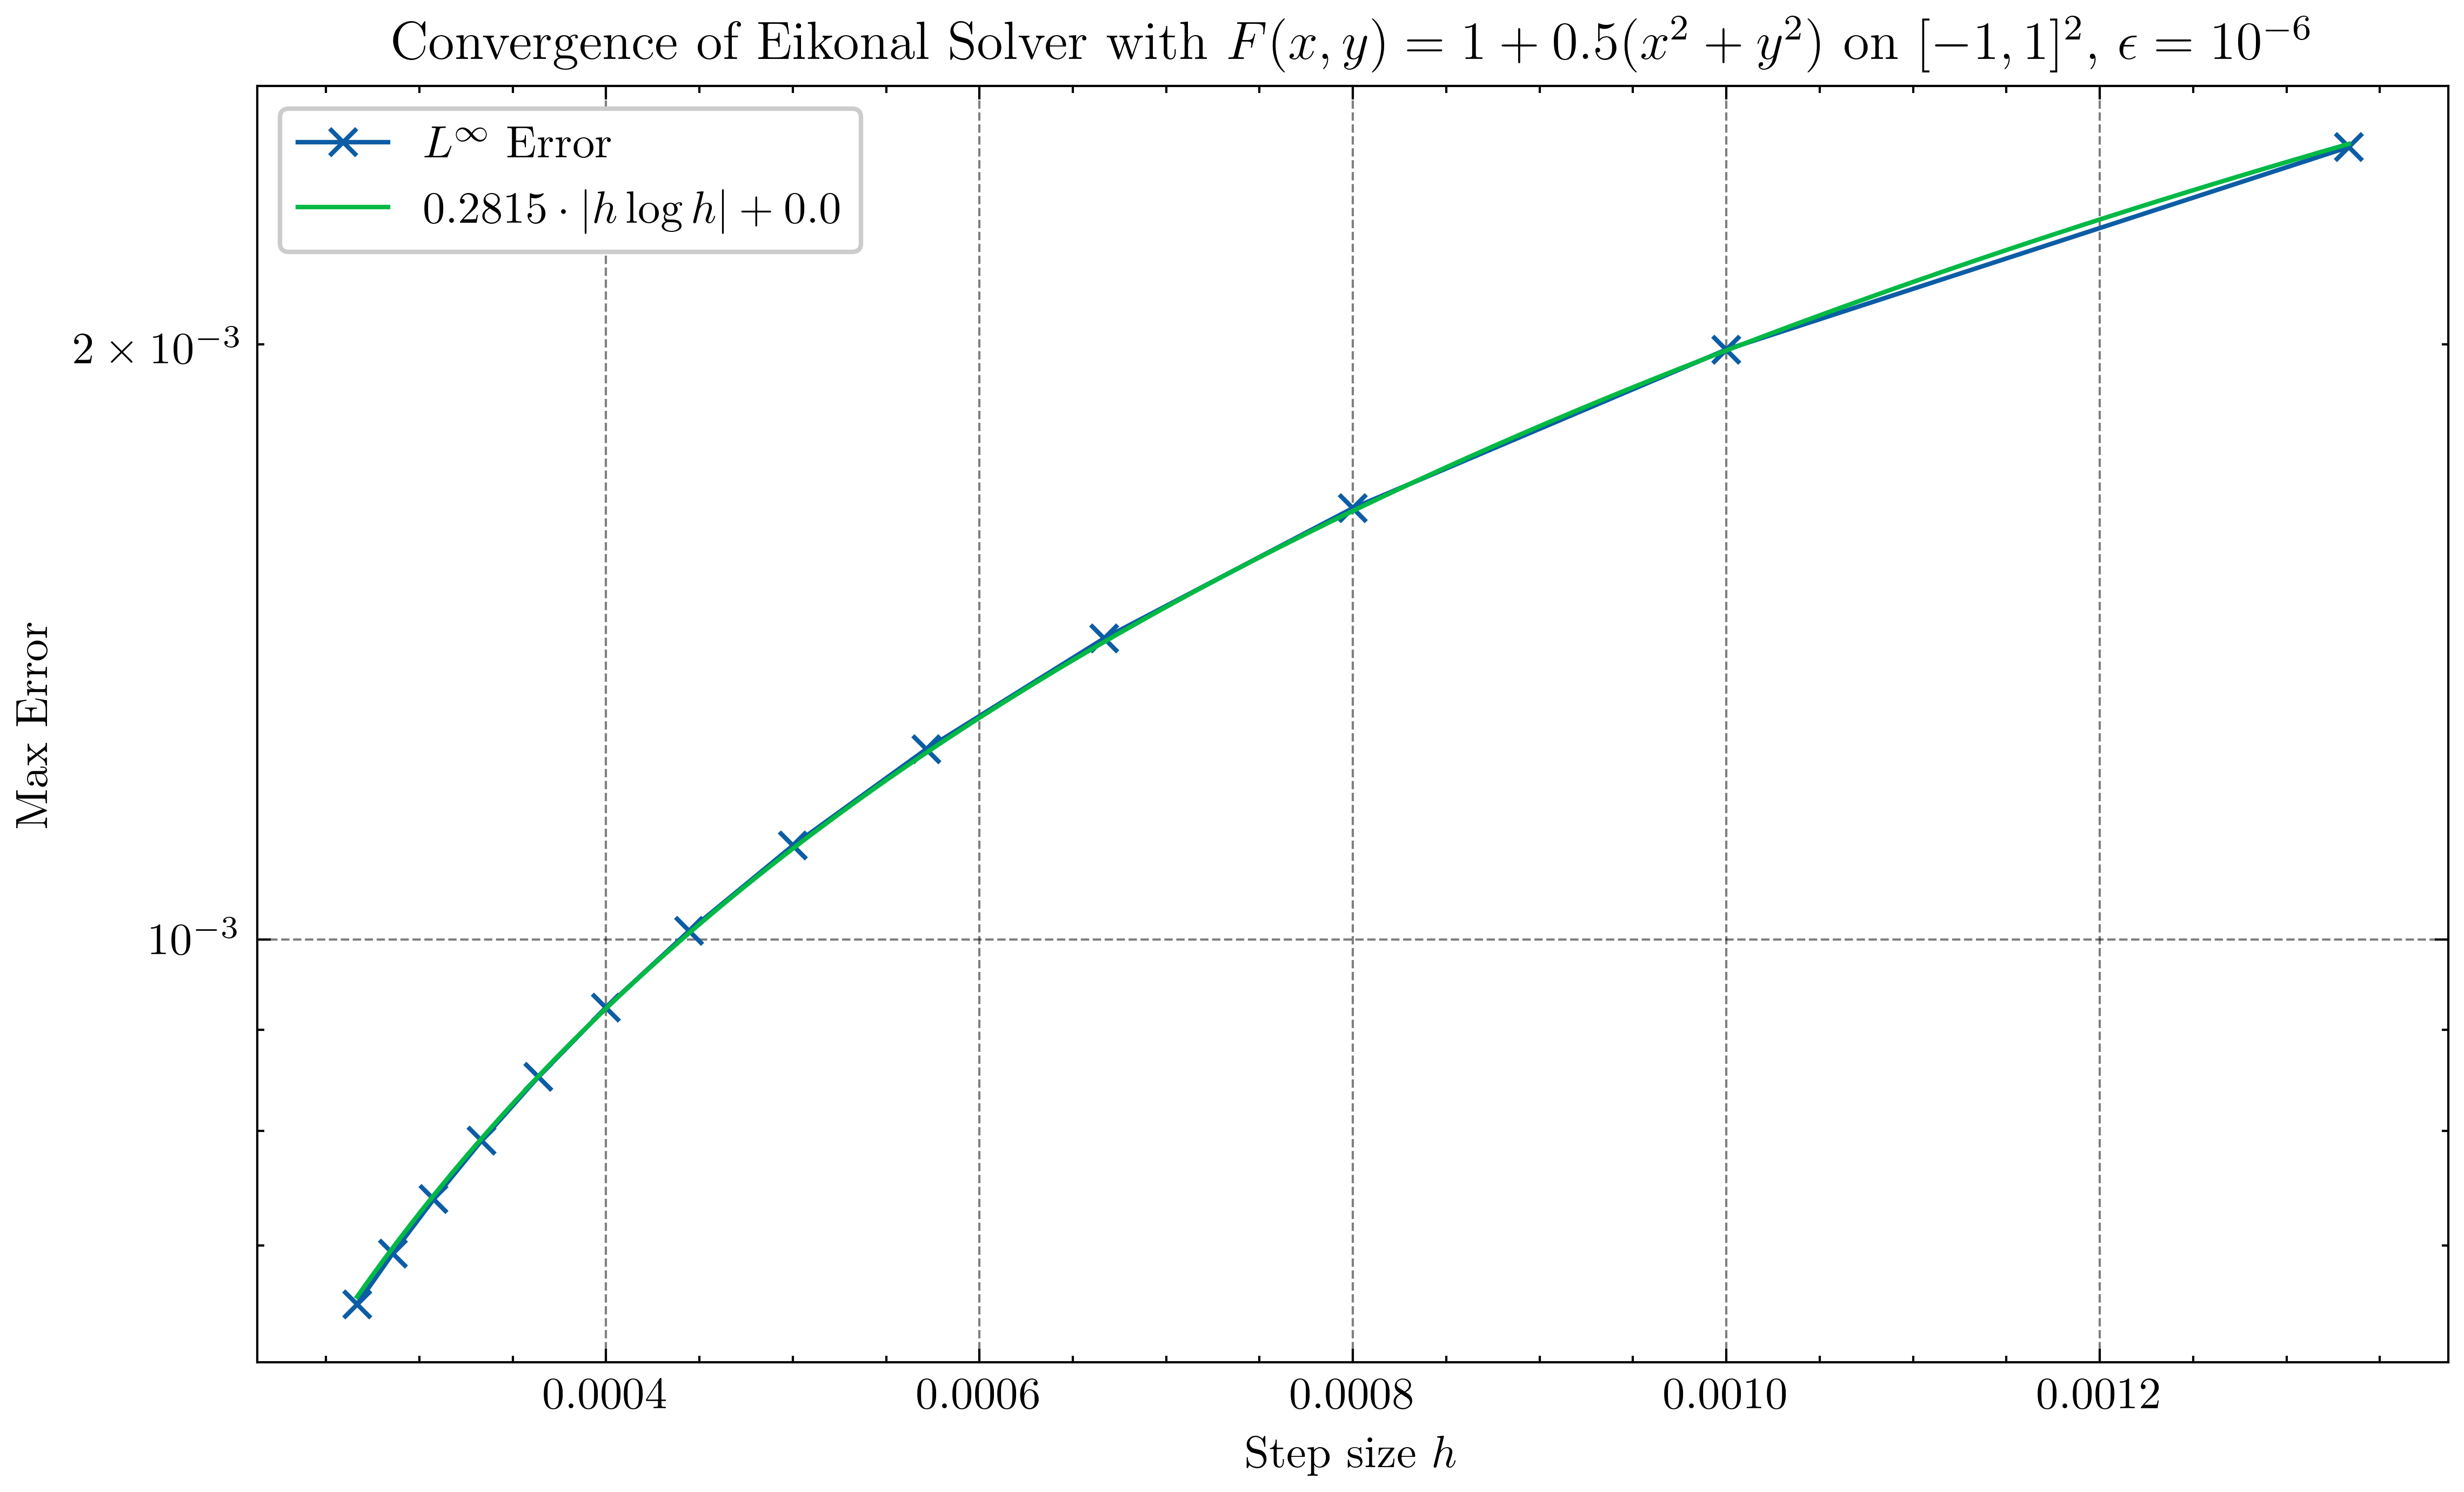
\includegraphics[width=0.6\textwidth]{plots/convergence2d_atan_step_size.png}
  \caption{Convergence plot}
  \label{fig:convarctan}
\end{figure}

\vspace{10pt}



\newpage

\section{An application of Eikonal equations : Path planning}
\label{path_planning}
In this section, we make use of the fast-sweeping method discussed to bridge our solutions with an application : path planning. Our goal is to compute an optimal path over a domain $\Omega\subset\R^2$, starting at a point $X_0\in \R^2$ to a target set $\Gamma$. \\
In particular, one can show in optimal control theory that given the Eikonal equation set-up that we described above where $F(x,y)$ is the positive function defining the "velocity" inside, say a medium, then the shortest path in time $\textbf{X}(t)\subset \R^2$ that goes from $X_0$ to $\Gamma$ must satisfy the following diffential equation:
\begin{equation}
\label{general_form_optimal_path_DE}
    \frac{d\textbf{X}(t)}{dt}=-\nabla u(\textbf{X}(t)), \quad \textbf{X}(0)=X_0
\end{equation}

\noindent where $u$ is the solution to the Eikonal equation (\ref{original-eikonal}). In 2D, equation (\ref{general_form_optimal_path_DE}) can be rewritten as : 

\begin{equation}
\label{optimal_path_DE_2D}
    \begin{bmatrix}
        \dot{x_1}(t) \\
        \dot{x_2}(t)
    \end{bmatrix} = \begin{bmatrix}
        -\partial_xu(x_1(t),x_2(t)) \\
        -\partial_yu(x_1(t),x_2(t))
    \end{bmatrix}
\end{equation}

\noindent Several points need to be taken care of. First, observe that (\ref{optimal_path_DE_2D}) is a time-continuous problem, while the solution $u$ obtained with the fast-sweeping method is discretized over a mesh with stepsize $h$. Therefore, we will need to be able to interpolate $\nabla u$ inside the cells of a mesh grid. For this, we will use bilinear interpolation. Secondly, we will have to discretize (\ref{optimal_path_DE_2D}) in order to solve the problem numerically.
\subsection{Bilinear interpolation}
Since our numerical solutions $u$ to Eikonal equations are available over a finite grid after using the Fast-Sweeping method, we need to be able to interpolate the values of the gradient of $u$ for points that do not lie in the grid, i.e. points that lie inside the cells of the grid. For this, we use bilinear interpolation. A visual explanation is displayed below.

\begin{figure}[h]
  \centering
  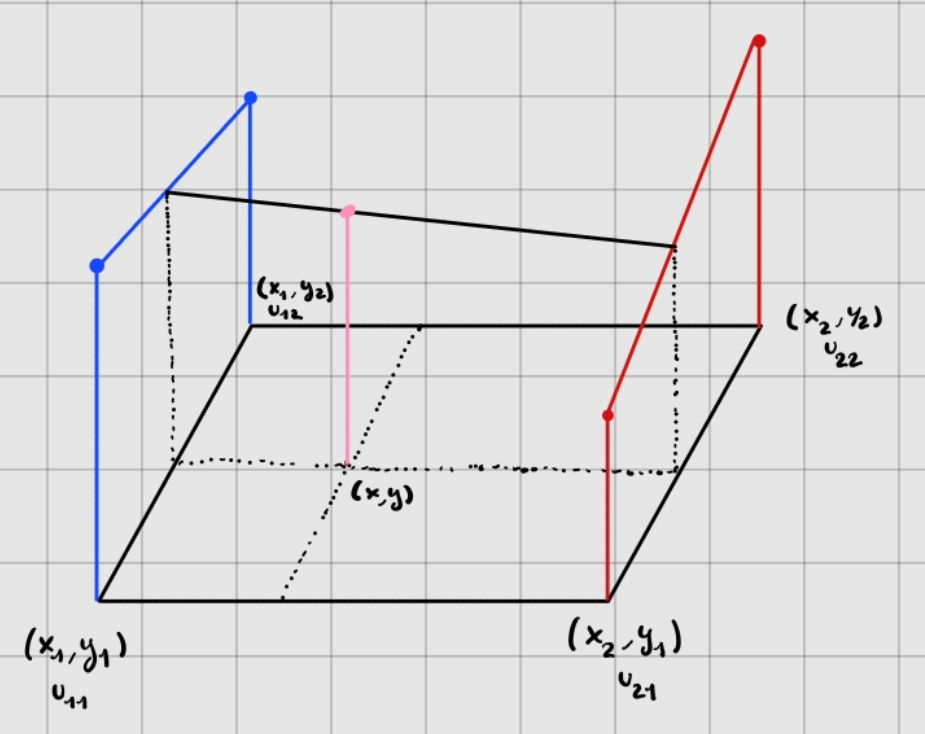
\includegraphics[width=0.5\textwidth]{bilinear_interpolation.jpg}
  \caption{Visual explanation of bilinear interpolation}
  \label{fig:your_label}
\end{figure}

\FloatBarrier

\noindent Given that we know the values $u_{11},u_{12},u_{21}$ and $u_{22}$, we can interpolate $u(x,y)$ inside the cell as follows.

\noindent The value of $u$ at the pink point on the graph above can be seen as a convex combination of the value of $u$ on the blue line ($x=x_1$) and the value of $u$ on the red line ($x=x_2$). Hence, our first step is to obtain these 2 values. Let:
\begin{equation*}
    \alpha=\alpha(y)=\frac{y-y_1}{y_2-y_1}
\end{equation*}
\noindent The interpolated value $u_b$ of $u$ on the blue line and the interpolated value $u_r$ of $u$ on the red line are respectively given by:
\begin{equation*}
    u_b=\alpha u_{11}+(1-\alpha)u_{12}, \quad u_r=\alpha u_{21}+(1-\alpha)u_{22}
\end{equation*}
From this point, we now let 
\begin{equation*}
    \beta=\beta(x)=\frac{x-x_1}{x_2-x_1}
\end{equation*}
\noindent and we can now compute the interpolated value at $\tilde{u}(x,y)$ as a convex combination of $u_b$ and $u_r$:
\begin{equation}
\label{interpolation}
    \tilde{u}(x,y)&=\beta u_b+(1-\beta)u_r \\
    &= \beta[\alpha u_{11}+(1-\alpha)u_{12}]+(1-\beta)[\alpha u_{21}+(1-\alpha)u_{12}]
\end{equation}
\noindent where the parameters $\alpha$ and $\beta$ are functions of $y$ and $x$ respectively. Therefore, we can take the derivatives of (\ref{interpolation}) w.r.t. $x$ and $y$, which is how we obtain the interpolated gradient of $u$.


\subsection{Discretization of the ODE system}
As discussed above, we approach the differential equation (\ref{optimal_path_DE_2D}) using a forward-in-time Euler discretization.Let $x_i^{n}=x_i(n\Delta t), i=1,2$. The scheme is:
\begin{equation}
    \begin{cases}
        \frac{x_1^{n+1}-x_1^n}{\Delta t}=-\Tilde{u_x}(x_1^n,x_2^n) \\
        \frac{x_2^{n+1}-x_2^n}{\Delta t}=-\Tilde{u_y}(x_1^n,x_2^n)
    \end{cases} \implies
    \begin{cases}
        x_1^{n+1} = x_1^n-\Delta t\Tilde{u_x}(x_1^n,x_2^n) \\
        x_2^{n+1} = x_2^n-\Delta t\Tilde{u_y}(x_1^n,x_2^n)
    \end{cases}
\end{equation}

\noindent which we recognize as being a gradient descent, stopping when $[x_1^n,x_2^n]^T\in \Gamma$, and where $\Tilde{u_x}$ and $\Tilde{u_y}$ are the interpolated first derivatives of the numerical solution $u$.

\subsection{Example : light refraction with Snell's law}
\label{section_snells_law}
This example covers the refraction of light when it crosses 2 media with different refraction indices. Indeed, some of the first appearances of the Eikonal equations appeared in this type of problems. Consider the following problem : we look at rays of lights in a square domain, where the lower half of the domain's refraction index is 2, and the index is 1 in the upper half plane. Suppose that light is emitted at the point $X_0$ and we want to know what is the path that the rays emitted at $X_0$ will take to get to $\Gamma$. By Fermat's principle, this path is unique and is the shortest in time. However, the change of medium will make the rays of light "change" direction at the interface. \\

\begin{center}
\begin{tikzpicture}[scale=4]
  % Domain outline
  \draw[thick] (0,0) rectangle (1,1);

  % Colored background rectangles for media
  \fill[blue!10] (0,0.5) rectangle (1,1);  % upper half (n = 1)
  \fill[orange!20] (0,0) rectangle (1,0.5);  % lower half (n = 2)

  % Interface line
  \draw[dashed, thick] (0,0.5) -- (1,0.5);

  % Medium labels
  \node at (0.25,0.75) {\large$n = 1$};
  \node at (0.75,0.10) {\large$n = 2$};

  % Source point X0
  \filldraw[blue] (0.4,0.2) circle (0.015) node[below left] {$X_0$};

  % Target Gamma point
  \filldraw[red] (0.8,0.85) circle (0.015) node[above right] {$\Gamma$};

  % Refracted path
  \draw[very thick, ->] (0.4,0.2) -- (0.48,0.5);
  \draw[very thick, ->] (0.48,0.5) -- (0.8,0.85);

  % Interface label
  \node[below right] at (0.001,0.5) {Interface};

\end{tikzpicture}
\end{center}

\noindent The refractive index $n=n(x,y)$ is inversely proportional to the speed in the medium. Hence, assume that we have solved the solution to (\ref{original-eikonal}) over $[-1,1]^2$, with $F(x,y)=F_2 =2$ in the lower half of $[-1,1]^2$, and $F(x,y)=F_1 = 1$ in the upper half. We know that in each medium, the path will consist of 2 straight lines that will join each other at the interface, on the line $y=0$. Therefore, one can compute the coordinates of the point $x$ which minimizes the time travel of light over the path from $X_0=(x_0,y_0)$ and the target $\Gamma=(x_T,y_T)$, i.e.:

\begin{equation}
\label{travel_time}
    \min_{x\in[-1,1]}T(x)=\underbrace{\frac{\sqrt{(x-x_0)^2+y_0^2}}{F_1}}_{\text{Time of travel in lower half}}+\underbrace{\frac{\sqrt{(x-x_T)^2+y_T^2}}{F_2}}_{\text{Time of travel in upper half}}
\end{equation}

\noindent Note that we strategically placed the interface on the line $y=0$, in order to simplify a bit this optimization problem. In our implementation, we chose $X_0=(x_0,y_0)=(0,-0.5)$ and $\Gamma =(0.5,0.5)$ which also simplifies the optimization problem. But we are still lazy and use \texttt{Scipy} in order to compute the solution to (\ref{travel_time}). \\
\noindent Our next step is to solve (\ref{optimal_path_DE_2D}), and compare our path to the true path which we obtained above by computing the $x$-coordinate of the intersection on the interface. We use the \texttt{solvers.ODE\_backtracer} method available in the repository and obtain the path below.

\begin{figure}[h]
  \centering
  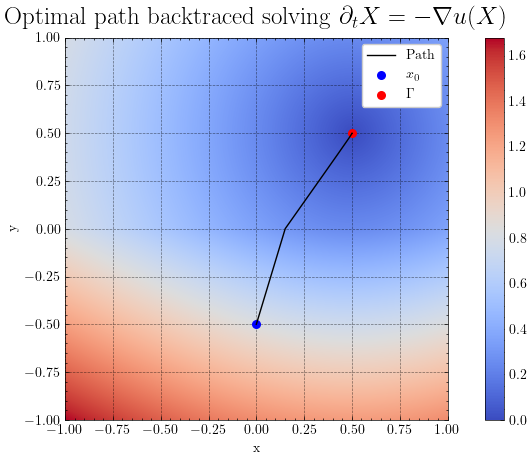
\includegraphics[width=0.48\textwidth]{plots/snell_path.png}
  \caption{Backtraced path from $X_0$ to $\Gamma$ using the numerical solution to the ODE system (\ref{optimal_path_DE_2D})}
  \label{fig:snell_path}
\end{figure}

\FloatBarrier

\noindent This path seems correct but we would like to confirm that our implementation does converge to the true solution. Luckily, the previous work we did to compute the $x$-coordinate on the line $y=0$ can be compared with our path. For this purpose, we introduce the Hausdorff distance: \\

\vspace{5pt}

\noindent\textbf{Hausdorff distance between 2 curves :} Given 2 curves $S_1,S_2\subset \mathbb{R}^n$, the Hausdorff distance is a measure that quantifies how close the curves $S_1$ and $S_2$ are to each other in space. It is formally defined as: 
\begin{equation*}
    d_H(S_1,S_2)=\max\{\sup_{s_1\in S_1}d(s_1,S_2),\sup_{s_2\in S_2}d(S_1,s_2)\}
\end{equation*}
where $d(x,y)$ is a metric on $\R^2$. In our case, we consider the the Hausdorff distance using the Euclidean metric $d$. It holds that $d_H(S_1,S_2)=0\iff S_1=S_2$, and $S_n\xrightarrow{n\to\infty}S\iff\lim_{n\to\infty}d_H(S_n,S)=0$.
Therefore, after obtaining our true path using Snell's law, we solve the ODE problem with several values of $\Delta t$, and compute $d_H(S_{\Delta_t},S)$ where $S_{\Delta_t}$ denotes the numerical path computed, and $S$ denotes the true path computed with Snell's law. We expect $d_H(S_{\Delta_t},S)\xrightarrow{\Delta_t\to0}0$, and that is what we obtain indeed for $\Delta_t\in[1.75h,3h]$ \\

\begin{figure}[h]
  \centering
  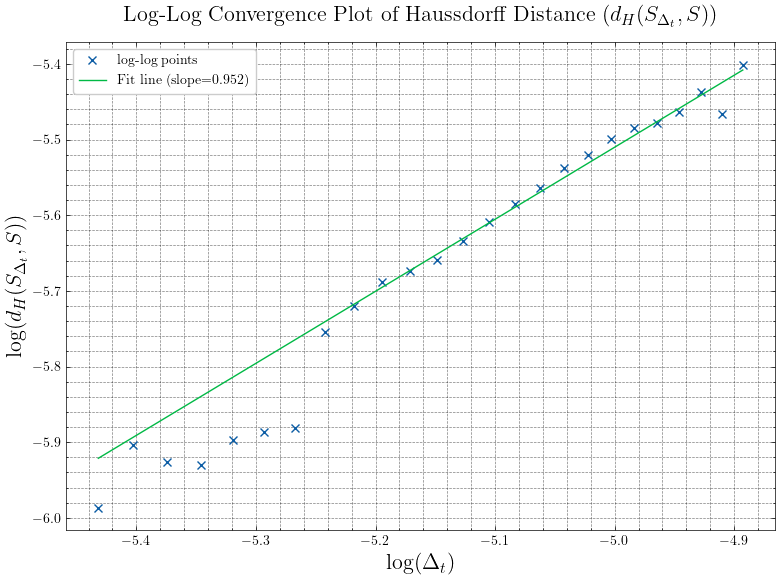
\includegraphics[width=0.7\linewidth]{plots/loglog_plot_convergence_path.png}
  \caption{Log-Log plot of the Hausdorff distance versus $\Delta t$}
  \label{fig:loglog_conv_hausdorff}
\end{figure} \\

\FloatBarrier

\noindent The green line was fitted on the 18 first points starting from the right. It had a slope roughly equal to 1, which was expected since the forward-in-time Euler discretization is of order $\mathcal{O}(\Delta_t)$. However, we notice that around $\log(\Delta_t)\approx-5.25$, there seems to be a drop in the log Hausdorff distance, and the errors seems to plateau beyond this point. We verify this assumption by plotting the error over a larger range ($\Delta_t\in[h,3h]$). \\

\begin{figure}[h!]
  \centering
  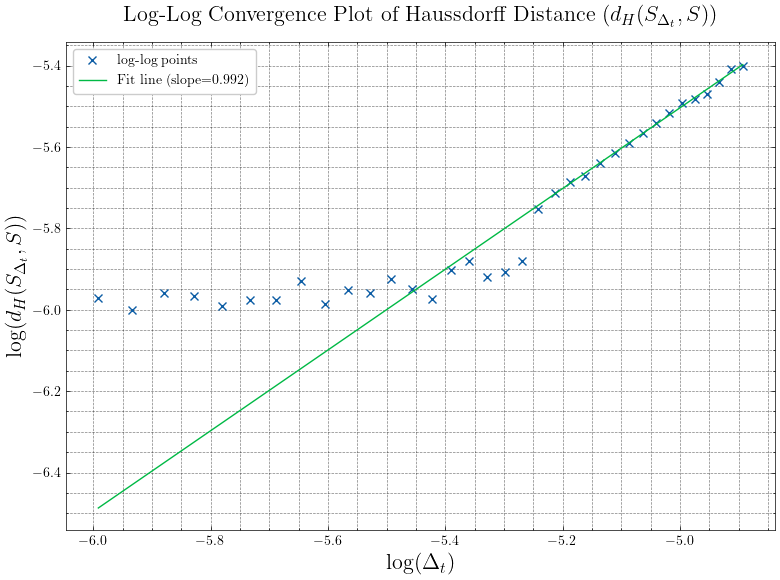
\includegraphics[width=0.7\linewidth]{plots/loglog_plot_convergence_path_larger_window.png}
  \caption{Log-Log plot of the Hausdorff distance versus $\Delta t$ on a larger window for $\Delta
  _t$}
  \label{fig:loglog_conv_hausdorff}
\end{figure} 

\FloatBarrier

\noindent Our claim is the following : even if our numerical ODE solver's accuracy is of order $\mathcal{O}(\Delta_t)$, this plateau probably occurs at a point, where it is now our bilinear interpolation which causes this error to plateau with respect to $\Delta_t$. In other words, after this , the error induced by lowering $\Delta_t$ is lower than the error induced by the bilinear interpolation.

\subsection{Paths avoiding objects}
In this final section, we use our path planning technique developped in the sections above on some more interesting examples. In the examples below, we let the velocity function $F(x,y)$ take different values on the different regions of the domain, set a starting point and a target and let our ODE solver compute the optimal path. These could be thought of as objects in a room, and the path would be a path computed by a robot, to go from its starting point $X_0$ to $\Gamma$

\begin{figure}[h]
  \centering
  \begin{minipage}{0.45\textwidth}
    \centering
    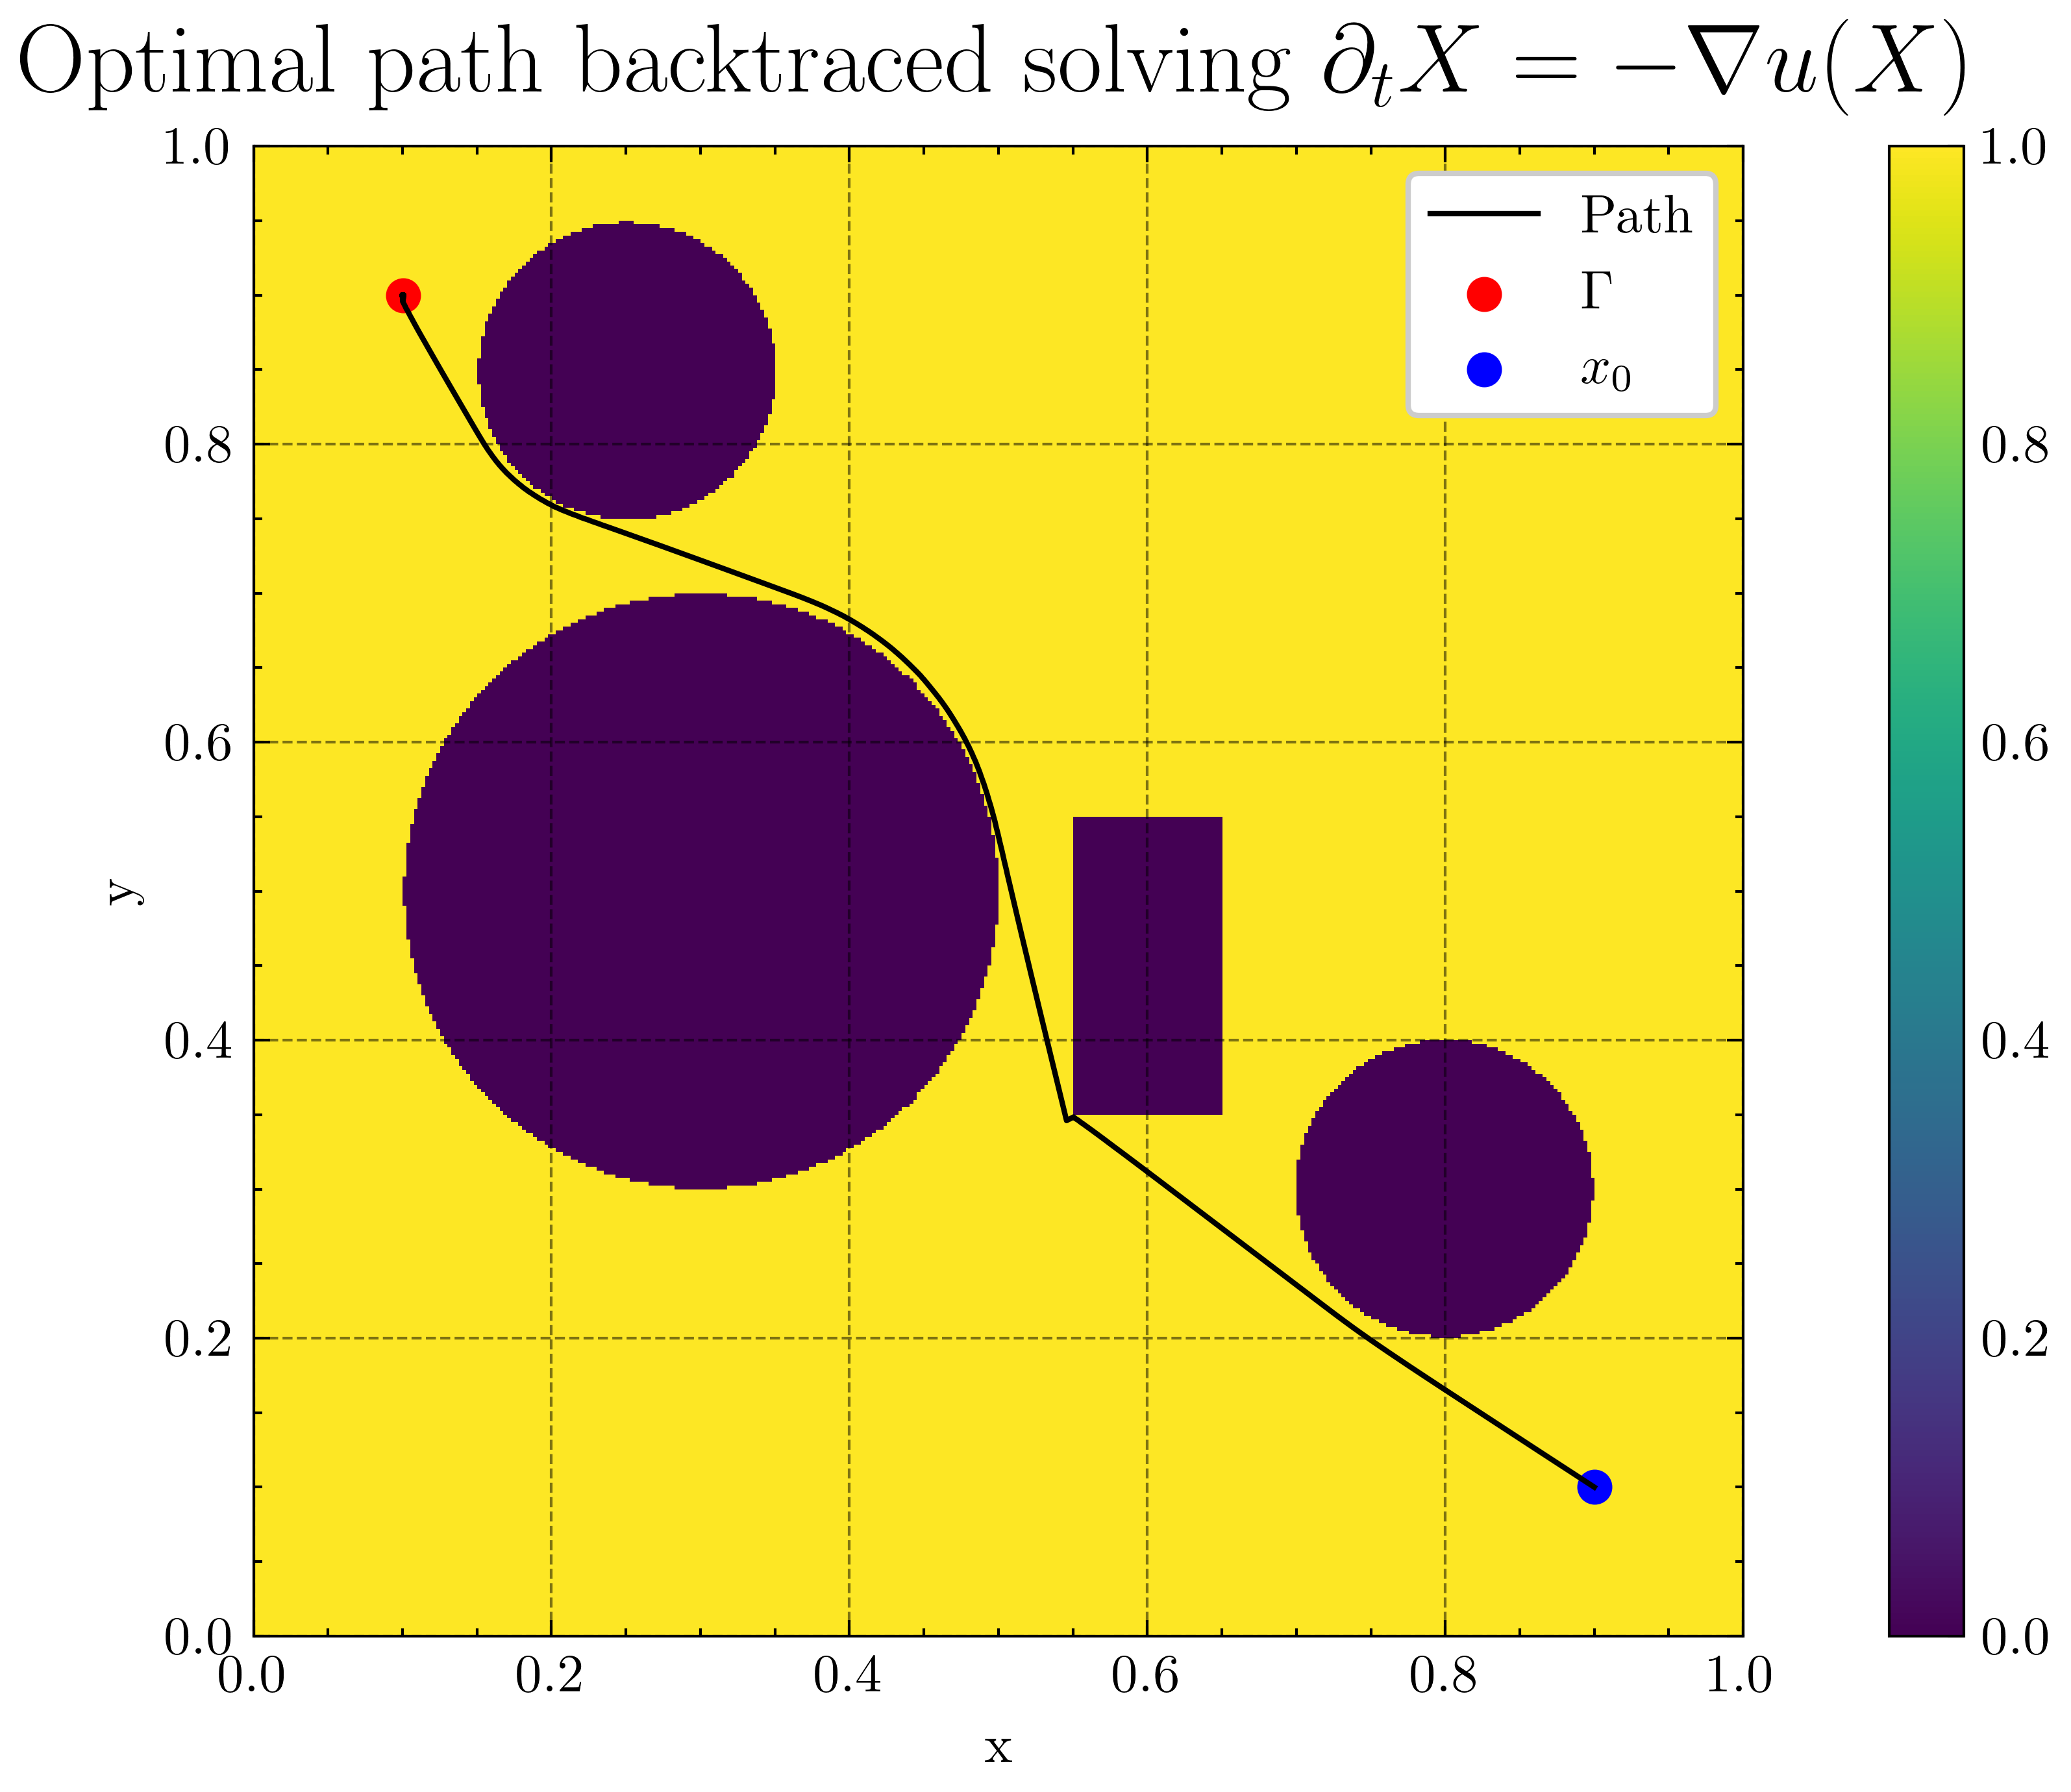
\includegraphics[width=\textwidth]{plots/path_mountain.png}
    \caption{Path backtraced on the domain, the heatmap represents the values of $F(x,y)$}
  \end{minipage}
  \hfill
  \begin{minipage}{0.45\textwidth}
    \centering
    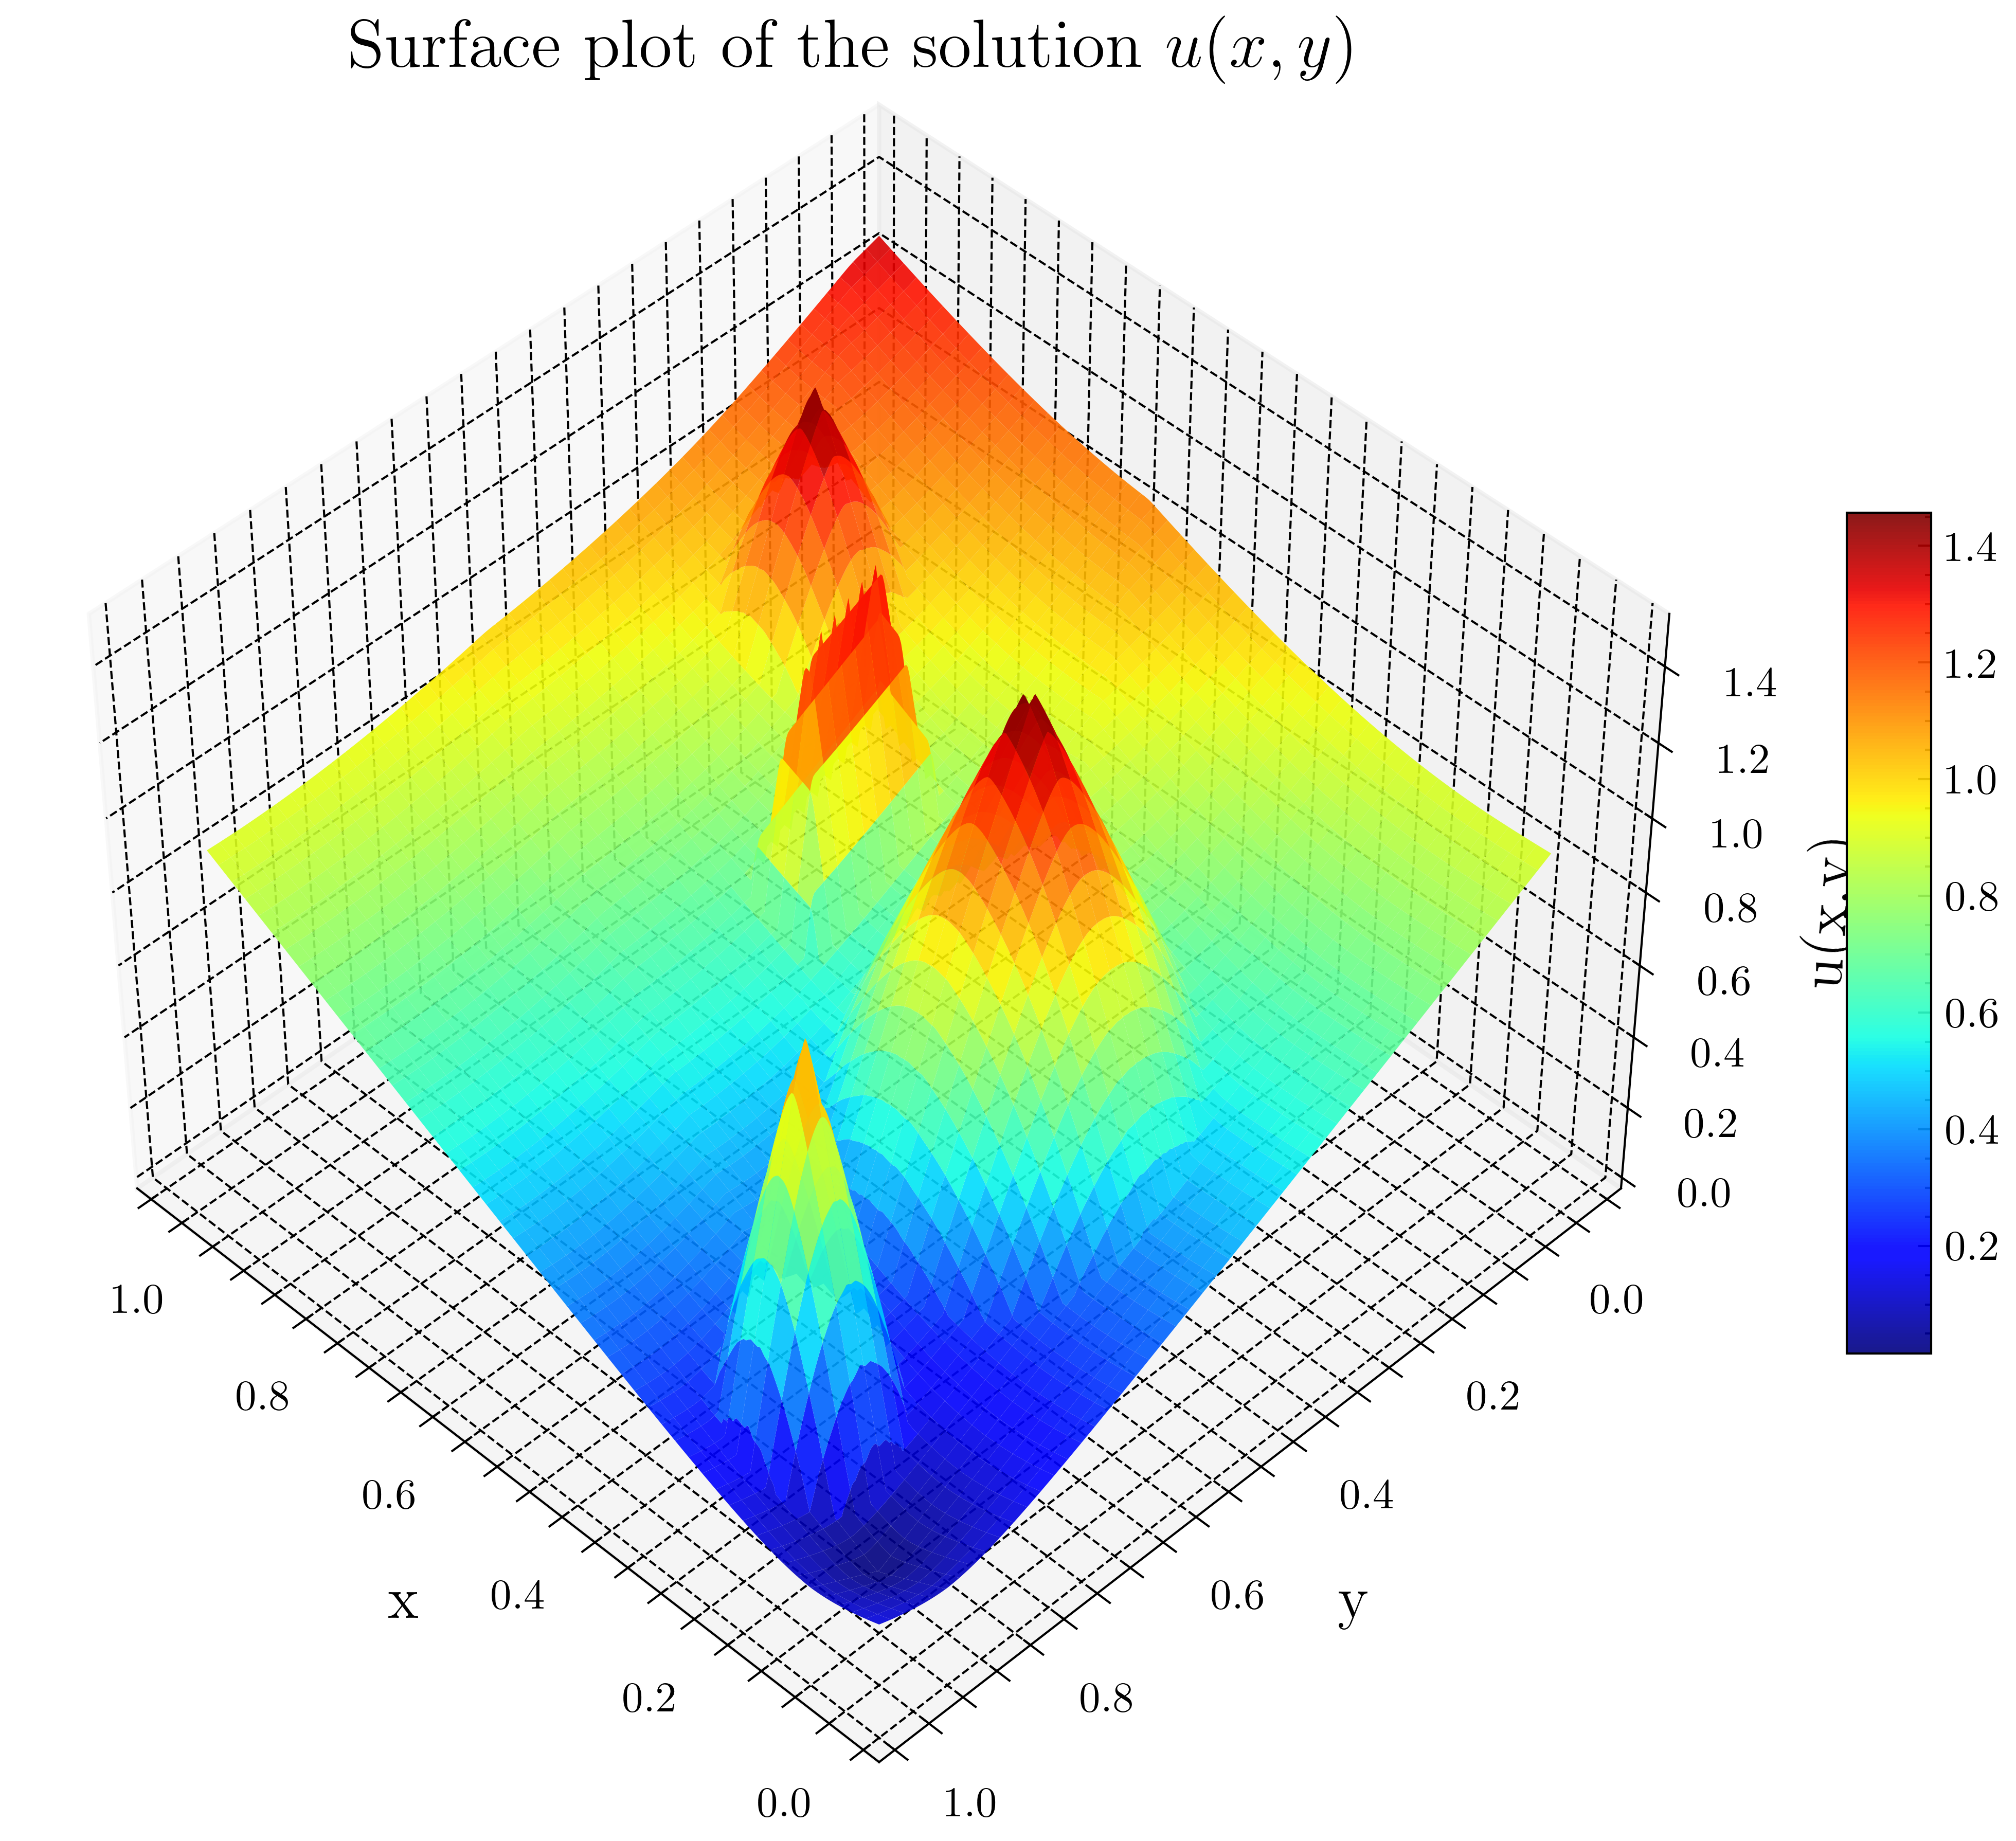
\includegraphics[width=\textwidth]{plots/surface_mountain.png}
    \caption{The 3D surface of the solution}
    \label{3d_surface_mountain}
  \end{minipage}
\end{figure}

\FloatBarrier

\begin{figure}[h]
  \centering
  \begin{minipage}{0.45\textwidth}
    \centering
    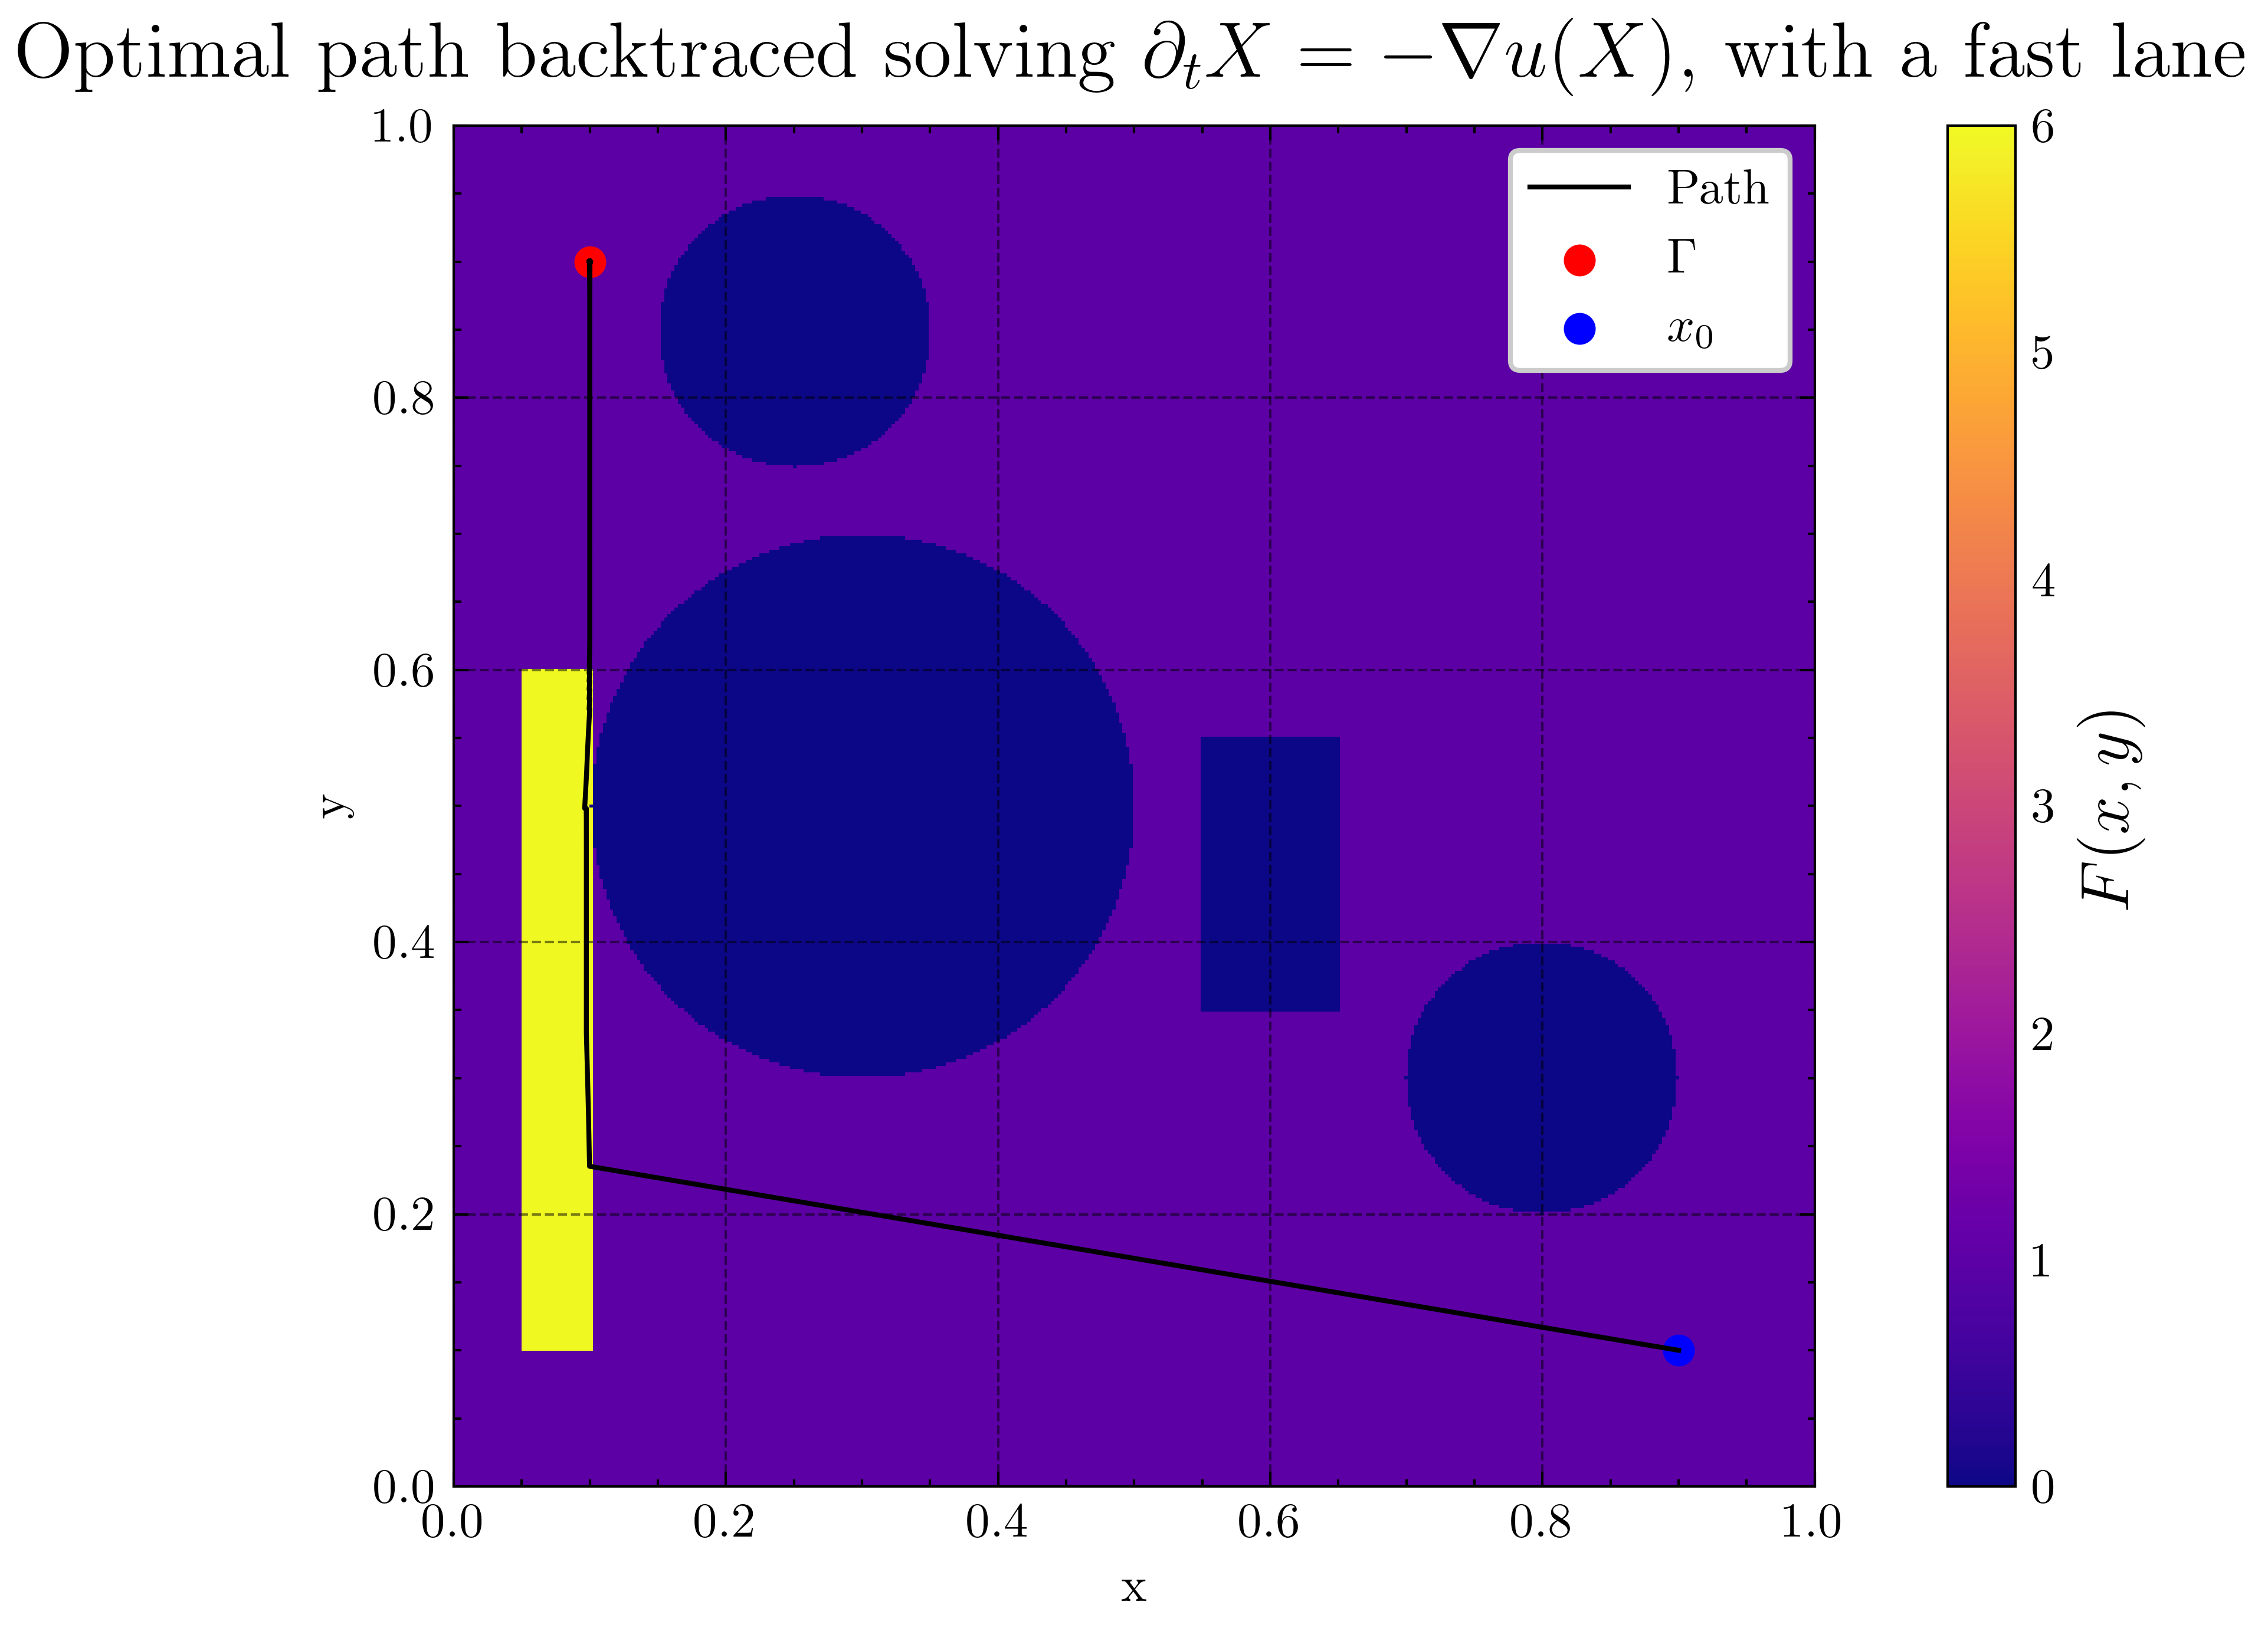
\includegraphics[width=\textwidth]{plots/path_mountain_fast_lane.png}
    \caption{Path backtraced on the domain, the heatmap represent the values of $F(x,y)$. Unlike above, we added a fast lane (yellow)}
  \end{minipage}
  \hfill
  \begin{minipage}{0.45\textwidth}
    \centering
    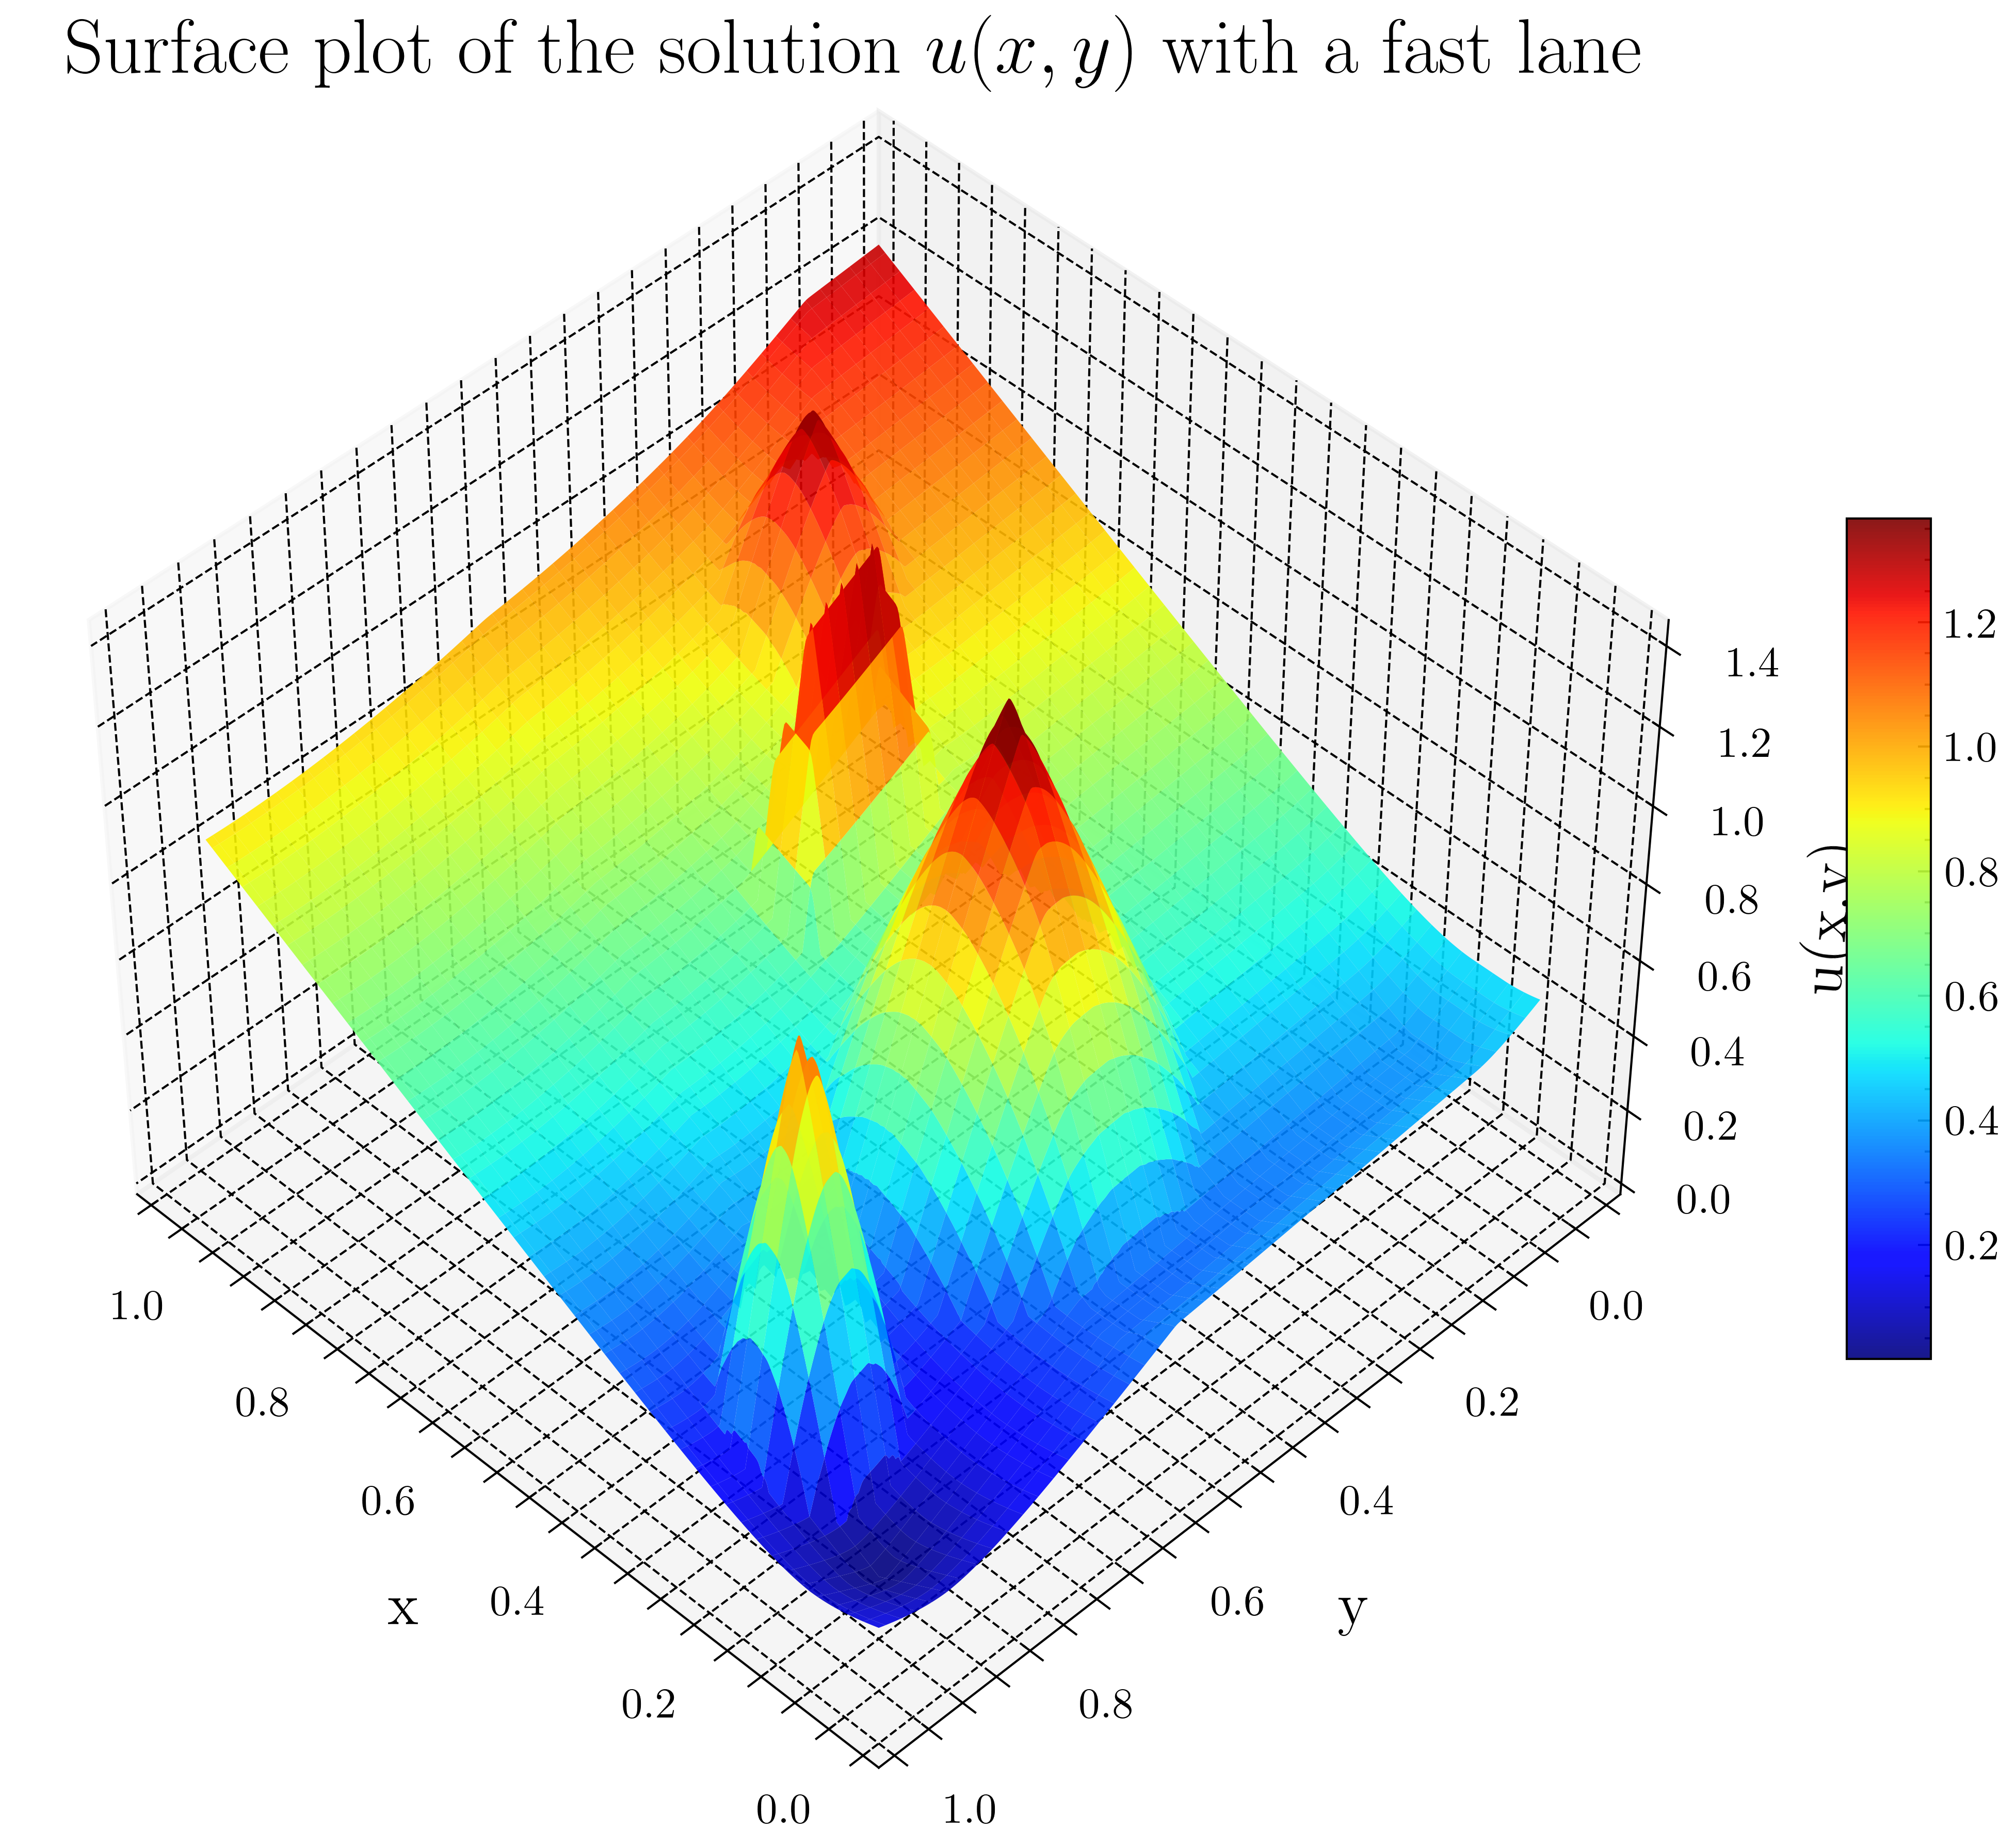
\includegraphics[width=\textwidth]{plots/surface_mountain_fast_lane.png}
    \caption{The 3D surface of the solution}
    \label{3d_surface_mountain_fast_lane}
  \end{minipage}
\end{figure}
\FloatBarrier

\noindent It is particularly interesting to see that the path indeed avoids these regions with low velocities, which can be visualized more easily on figure (\ref{3d_surface_mountain}). We introduced a "fast lane" in the second example, where we set $F(x,y)=6$, and this completely modifies the trajectory of the optimal path in time. Figures (\ref{3d_surface_mountain}) and (\ref{3d_surface_mountain_fast_lane}) are interesting to compare : adding the fast lane on the left side of the domain significantly lowers the value of $u$ in this region, i.e. the cost it takes to go from there to the target $\Gamma$.
Thanks to Madelyn Schaffer for her idea of introducing a fast-lane, and allowing me to adapt it to my example!
\section{Conclusion}
In this report, we aimed at implementing the Fast-Sweeping method for solving Eikonal equations. This Hamilton-Jacobi scheme can easily be extended to high-dimensional problems, and is not computationally too expensive. This method possesses several interesting properties, especially regarding its order of accuracy which heavily depends on the set-up the boundary-value problem. Several points could be addressed in further investigation of the fast-sweeping method. In particular, a few ideas we would like to investigate (and potentially update this report with) are :
\begin{itemize}
    \item Formalizing the orders of convergence of the method, especially when the velocity field $F$ is not constant or when $|\Gamma|>1$, mentioned in (\ref{prop_general_equations}). We would also want to look at the regime change of the order of accuracy when computing the distance functions with $|\Gamma|>1$.
    \item The accuracy of the Hausdorff distance in section (\ref{section_snells_law}) eventually reaches a plateau. We claim that higher-accuracy interpolation methods such as bicubic interpolation would help pushing this plateau to happen at lower values of $\Delta_t$, and thus help achieve better accuracies for the path computations. Similarly, we could use some other discretizations the ODE system, and obtain a better accuracy.
    \item We would also like to go over our Python implementation in order to optimize the algorithm and potentially decrease the runtime. This has been an iterative process since the beginning of this project, but there surely are opportunities left to lower the runtime.
    \item Finally, we would like to find some topographical data in order to apply our path planning to a real-life scenario. If we can get access to the elevation map of a specific region, we could compute the shortest path in time given these elevations. For example, the gradient of the terrain could be used to inform the velocity field $F$ (i.e. penalize the velocity when the norm of the gradient of the elevation is high).
\end{itemize}

\begin{thebibliography}{9}

\bibitem{zhao2005}
H. Zhao, 
\textit{A fast sweeping method for Eikonal equations},
Mathematics of Computation, 74(250):603–627, 2005.

\bibitem{wiki-eikonal}
Wikipedia contributors, 
\textit{Eikonal equation}, 
Wikipedia, The Free Encyclopedia, 
\href{https://en.wikipedia.org/wiki/Eikonal_equation}{https://en.wikipedia.org/wiki/Eikonal\_equation}.

\bibitem{numpy}
Harris, Charles R., et al. 
\textit{Array programming with NumPy}. 
Nature 585, 357–362 (2020).


\end{thebibliography}

\end{document}


